% ------------------------------------------------------------------------
% ------------------------------------------------------------------------
% Modelo de Trabalho Acadêmico utilizando repUERJ 
% tese de doutorado, dissertação de mestrado e trabalhos monográficos em geral
%
% * Este aquivo está editado na codificação de caracteres UTF-8.
%
% ------------------------------------------------------------------------
% ------------------------------------------------------------------------
%
\documentclass[a4paper,12pt,oneside,onecolumn,final,fleqn]{repUERJ}

% ---
% Pacotes fundamentais 
% ---
\usepackage[brazil]{babel}  % adequacao para o portugues Brasil
\usepackage[utf8]{inputenc} % Determina a codificacao utiizada
                            % (conversão automática dos acentos)
\usepackage{makeidx}        % Cria o indice
\usepackage{hyperref}       % Controla a formacao do indice
\usepackage{lastpage}       % Usado pela Ficha catalografica
\usepackage{indentfirst}    % Indenta o primeiro paragrafo de cada secao.
\usepackage{xcolor}          % Controle das cores
\usepackage{graphicx}       % Inclusao de graficos
\usepackage{subfig}
\usepackage{amsmath}        % pacote matemático
\usepackage{amssymb}
\usepackage{amsthm}
\usepackage{hhline}
\usepackage{tikz}
\usetikzlibrary{calc}
\usepackage{multirow}
\usepackage{bigstrut}
\usepackage{algpseudocode}



\usepackage{setspace}
\usepackage{caption}
\captionsetup[table]{singlelinecheck=false}
\captionsetup[figure]{slc=off}
\captionsetup{font=singlespacing}
\captionsetup{tableposition=top}

\theoremstyle{plain}
\newtheorem{thm}{Theorem}[chapter] % reset theorem numbering for each chapter

\theoremstyle{definition}
\newtheorem{defn}[thm]{Definition} % definition numbers are dependent on theorem numbers
\newtheorem{exmp}[thm]{Example}

\usepackage{macrosfabbri-basic}
\usepackage{macrosfabbri-dg}
\newcommand{\RNum}[1]{\uppercase\expandafter{\romannumeral #1\relax}}
\newcommand{\rnum}[1]{\expandafter{\romannumeral #1\relax}}
\renewcommand{\myparagraph}{\noindent\textbf}
\usepackage{forloop}
\newcounter{ct}
\newcommand{\markdent}[1]{\forloop{ct}{0}{\value{ct} < #1}{\hspace{\algorithmicindent}}}
\newcommand{\markcomment}[1]{\Statex\markdent{#1}}

% ---
% Pacote auxiliar para as normas da UERJ
% ---
\usepackage[frame=no,algline=yes,font=default]{repUERJformat}
% ---
% Pacotes de citacoes
% ---
\usepackage[alf]{abntex2cite}

% *****************************************************************************
% *****************************************************************************
% Comandos especificos deste exemplo 
% * podem ser retirados na edicao de um novo documento
% *****************************************************************************
% *****************************************************************************

\newcommand{\comando}[1]{\texttt{\bs #1}}
\newcommand{\opcoes}[1]{\texttt{[}\textsl{#1}\texttt{]}}
\newcommand{\param}[1]{\texttt{\{}\textsl{#1}\texttt{\}}}
\newcommand{\BibTeX}{{{Bib}}\TeX}
\newcommand{\repUERJ}{\textsf{repUERJ}}
\newcommand{\formato}[1]{\begin{flushleft}{#1}\end{flushleft}}
\newcommand{\bs}{\textbackslash}
\def\ReduceAfterCaptionfigspace{}

% *****************************************************************************
% *****************************************************************************
% Informacoes de autoria e institucionais
% *****************************************************************************
% *****************************************************************************

%-----------------------------------------------------------------------
% Imagens pretextuais (precisam estar no mesmo diretorio deste arquivo .tex)
%-----------------------------------------------------------------------

\logo{logo_uerj_cinza.png}
\marcadagua{marcadagua_uerj_cinza.png}{1}{160}{255}
%-----------------------------------------------------------------------
% Informacoes da instituicao
%-----------------------------------------------------------------------

\instituicao{Universidade do Estado do Rio de Janeiro}
            {Instituto Politécnico} 
            {Departamento de Modelagem Computacional}  
            {}

%-----------------------------------------------------------------------
% Informacoes da autoria do documento
%-----------------------------------------------------------------------

\autor{Pedro Felipe Pena}{Barata}
\titulo{Aplicações de técnicas atuais em reconstrução 3D fotogramétrica}

\palavraschaves{Fotogrametria}{Estrutura por Movimento}{Estereoscopia Multiocular}{Reconstrução 3D}

\title{Applications of current photogrammetric 3D reconstruction techniques}
\keywords{Photogrammetry}{Structure from Motion}{Multiview Stereo}{3D Reconstruction}

\orientador{Prof.\ Dr.} 
           {Ricardo}{Fabbri} 
           {Departamento de Modelagem Computacional -- UERJ}

%-----------------------------------------------------------------------
% Titulacao (Doutor, Mestre, Bacharel, Licenciado) e Curso
%-----------------------------------------------------------------------

\grau{Graduado}  
\curso{Engenharia de Computação} 
\areadeconcentracao{}

%-----------------------------------------------------------------------
% Informacoes adicionais (local, data e paginas)
%-----------------------------------------------------------------------

\local{Nova Friburgo} 
\data{23}{Novembro}{2017} 

% *****************************************************************************
% *****************************************************************************
% Configurações de aparência do PDF final
% *****************************************************************************
% *****************************************************************************

% alterando o aspecto da cor azul
\definecolor{blue}{RGB}{41,5,195}
\definecolor{apricot}{RGB}{251,206,177}

% informações do PDF
\hypersetup{
  %backref=true,
  %pagebackref=true,
  %bookmarks=true,                  % show bookmarks bar?
  unicode=false,
  pdftitle={\UERJtitulo},
  pdfauthor={\UERJautor},
  pdfsubject={\UERJpreambulo},
  pdfkeywords={PALAVRAS}{CHAVES}{\chaveA}{\chaveB}{\chaveC}{\chaveD},
  pdfproducer={\packagename}, % producer of the document
  pdfcreator={\UERJautor},
  colorlinks=true,                  % false: boxed links; true: colored links
  linkcolor=blue,                   % color of internal links blue
  citecolor=red,                    % color of links to bibliography blue
  filecolor=magenta,                % color of file links magenta
  urlcolor=green,
  bookmarksdepth=4
}

% *****************************************************************************
% *****************************************************************************
% Início do documento
% *****************************************************************************
% *****************************************************************************

% ---
% compila o indice
% ---
\makeindex
% ---

% *****************************************************************************
% *****************************************************************************

\begin{document}
\pagestyle{empty}
\begin{tikzpicture}[overlay,remember picture]
    \draw [line width=2pt ]
        ($ (current page.north west) + (2cm,-2cm) $)
        rectangle
        ($ (current page.south east) + (-1cm,1.5cm) $);
    \draw [line width=1pt]
        ($ (current page.north west) + (2.1cm,-2.1cm) $)
        rectangle
        ($ (current page.south east) + (-1.1cm,1.6cm) $);
\end{tikzpicture}
% ----------------------------------------------------------
% ELEMENTOS PRE-TEXTUAIS
% ----------------------------------------------------------

\frontmatter

% ----------------------------------------------------------
% Capa e a folha de rosto
% ----------------------------------------------------------

\capa
\pagestyle{empty}
\begin{tikzpicture}[overlay,remember picture]
    \draw [line width=2pt ]
        ($ (current page.north west) + (2cm,-2cm) $)
        rectangle
        ($ (current page.south east) + (-1cm,1.5cm) $);
    \draw [line width=1pt]
        ($ (current page.north west) + (2.1cm,-2.1cm) $)
        rectangle
        ($ (current page.south east) + (-1.1cm,1.6cm) $);
\end{tikzpicture}

\folhaderosto % modelo de folha de rosto para monografia do Inst. Fís. UERJ

% ----------------------------------------------------------
% Inserir a ficha catalografica
% ----------------------------------------------------------

%\fichacatalografica{fichacatalografica.pdf}

% ----------------------------------------------------------
% Folha de aprovacao
% ----------------------------------------------------------

\begin{folhadeaprovacao}
  \assinatura{Prof.\ Dr.\ Edirlei Soares -- UERJ}
  \assinatura{Prof.\ Dr.\ Roberto Pinheiro -- UERJ}

\end{folhadeaprovacao}

% ----------------------------------------------------------
% Dedicatoria
% ----------------------------------------------------------

%\pretextualchapter{Dedicatória}

%\vfill

% ----------------------------------------------------------
% Agradecimentos
% ----------------------------------------------------------

\pretextualchapter{Agradecimentos}

A Deus por ter me dado saúde e força para superar as dificuldades.


Á minha família por sempre me apoiar, até nos momentos mais dificeis.


Á UERJ e todo seu corpo docente, além da direção e administração, que mesmo sem ter condições ideais de funcionamento, realizam seu trabalho com tanto amor e dedicação, trabalhando incansavelmente para que nós, alunos, possamos contar com um ensino de extrema qualidade.


Ao meu professor e orientador Ricardo Fabbri, pelo suporte no pouco tempo que lhe coube, pelas suas correções e incentivos.

% ----------------------------------------------------------
% Epigrafe
% ----------------------------------------------------------

\pretextualchapter{}

  \vfill\
  \begin{flushright}
 Talvez não tenha conseguido fazer o melhor, mas lutei para que o melhor fosse feito. Não sou o que deveria ser, mas Graças a Deus, não sou o que era antes. \\
    \textsl{Marthin Luther King}
  \end{flushright}

% ----------------------------------------------------------
% RESUMO
% ----------------------------------------------------------

\pretextualchapter{Resumo}

\referencia

A área de reconstrução 3D vem sido amplamente explorada. Sensores de
profundidade, tanto aéreos quanto terrestres, têm sido empregados em diferentes
aplicações já há muito tempo. Entretanto, constantes melhorias na tecnologia, sobretudo, no
\emph{hardware} e \emph{software} no âmbito da reconstrução, fizeram com que
nas últimas duas décadas, novas técnicas surgissem.

Muitos cientistas que utilizavam a fotogrametria pura -- isto é, usando sensores de 
imagens convencionais -- haviam convertido seus esforços à área dos sensores a \emph{laser}. Além de
executarem uma reconstrução mais rápida e confiável de objetos com baixa
textura, tais sensores possuem uma altíssima acurácia, compensando seu alto
custo inicial.  Isto dificultou e desacelerou o processo de descoberta de novos
algoritmos e métodos em fotogrametria pura.

Graças a avanços recentes, a fotogrametria, aliada a novos algoritmos,
como o \emph{Structure from Motion} (SfM), pontos de interesse e o casamento entre
imagens, por exemplo, consegue competir com escaneadores a \emph{laser} e sensores de
profundidade. As características mais bem-reconhecidas das técnicas recentes, no
entanto, são a robustez, flexibilidade, e praticidade, não sendo claro se na prática podem 
competir com escaneadores a \emph{laser} quanto à precisão em aplicações de interesse.

Neste trabalho, investiga-se a praticidade de técnicas atuais combinando SfM e MVS
(\emph{Multi-View Stereo}), utilizando \emph{softwares} como o MVE~\cite{mve} e
o VisualSfM~\cite{wu2011visualsfm}. Em particular, relata-se um estudo de até
onde é possível chegar apenas utilizando-se a câmera de um \emph{smartphone}, visando
aplicação futura à preservação completa do patrimônio do Jardim do Nêgo, em Nova Friburgo.
Essa tecnologia é confrontada com outros tipos de técnicas empregadas em
grandes projetos, como o Kinect, da Microsoft, e sua aplicação em SfM, bem como técnicas clássicas de 
escaneamento a \emph{laser}, tais como as empregadas no projeto \emph{Digital Michelangelo} de preservação de
esculturas liderado pela Universidade de Stanford.


% O trabalho foi estruturado da seguinte maneira: previamente apresentam-se os objetivos do projeto, destacando suas funcionalidades e metas, a seguir divide-se em capítulos; O Capítulo 1, que introduz o funcionamento de cada algoritmo e técnica empregada, apresentando e debatendo, comparativamente pontos à favor e contra; O Capítulo 2 é dedicado à ferramenta gráfica utilizada para a obtenção dos resultados (VisualSfM). Finalmente, apresentamos os resultados e conclusões do trabalho, bem como sugestões para implementações e trabalhos futuros.

% ABORDAR OS "TODO'S" DO HANGOUTS


\imprimirchaves

% ----------------------------------------------------------
% Abstract
% ----------------------------------------------------------

\pretextualchapter{Abstract}

\reference

The field of 3D reconstruction has been widely explored. Range sensors, both aerial
and terrestrial, have long been employed in different applications. However, constant
improvements in technology, especially in hardware and software in the context
of reconstruction, have led to the emergence of new techniques in the past two decades.

Many scientists that used pure photogrammetry -- \ie, using conventional
imaging sensors -- have converted their efforts into the area of laser sensors.
Such sensors, beyond providing a faster and more reliable reconstruction for
objects with low texture information, provide high accuracy, justifying their
initial cost.  This hindered and slowed down the process of discovering new algorithms
and methods in pure photogrammetry.

Thanks to recent advances, photogrammetry, coupled with new algorithms
such as Structured Motion (SfM), interest points and image matching, for instance,
can compete with laser scanners and other range sensors. While Recent techniques are well-known for robustness, flexibility and ease of use, it is not yet clear whether they can compete with laser scanners in terms of precision in applications of interest.

In this work, we investigate the practical applicability of current techniques
combining SfM and MVS (\emph{Multi-View Stereo}), using softwares such as
MVE~\cite{mve} and VisualSfM~\cite{wu2011visualsfm}. In particular, we study
how far can one go by using a standard smartphone camera, aiming at a future application to the complete preservation of the sculpture garden Jardim do Nêgo at Nova Friburgo. 
This technology will be confronted against other types of techniques employed in
major projects, such as Microsoft's Kinect and its application in SfM, as well as
classical techniques of laser scanning of sculptures, such as those employed in
the Digital Michelangelo project, lead by Stanford University.

% The work was structured in the following way: previously presented the objectives of the project, highlighting its functionalities and goals, then divided into chapters; Chapter 1, which introduces the operation of each algorithm and technique employed, presenting and debating, comparatively points for and against; Chapter 2 is devoted to the graphing tool used to obtain the results (VisualSfM). Finally, we present the results and conclusions of the work, as well as suggestions for future implementations and work.


\printkeys

% ----------------------------------------------------------
% Listas de ilustrações e tabelas
% ----------------------------------------------------------

\listadefiguras
%\listadetabelas

% ----------------------------------------------------------
% Outras listas
% ----------------------------------------------------------

%\listadealgoritmos

% ----------------------------------------------------------
% Lista de abreviaturas e siglas
% ----------------------------------------------------------

%\pretextualchapter{Lista de abreviaturas e siglas}

% \abreviatura{ABNT}{Associação Brasileira de Normas Técnicas}

% ----------------------------------------------------------
% Lista de simbolos
% ----------------------------------------------------------

%\pretextualchapter{Lista de símbolos}

% \simbolo{\lambda_i}{i-ésimo autovalor}

% ----------------------------------------------------------
% Sumario
% ----------------------------------------------------------

\sumario


% ----------------------------------------------------------
% ELEMENTOS TEXTUAIS
% ----------------------------------------------------------

\mainmatter

%======================================================================================
\chapter{Introdução} \label{cap:intro}
%======================================================================================

\section*{Introdução e Justificativa}

A reconstrucão 3D de cenas gerais a partir de múltiplos pontos de vista
usando-se câmeras convencionais, sem aquisição controlada, é um dos grandes
objetivos de pesquisa em visão computacional, ambicioso até mesmo para os dias
de hoje. Aplicações incluem a reconstrução de modelos 3D para uso em
videogames~\cite{ablan2007digital}, filmes~\cite{ablan2007digital},
arqueologia, arquitetura, modelagem 3D urbana (\eg, Google Streetview); técnicas
de \emph{match-moving} em cinematografia para fusão de conteúdo virtual e
filmagem real~\cite{dobbert2012matchmoving}, a organização de uma coleção de
fotografias com relação a uma cena (\eg, o sistema
\emph{Phototourism}~\cite{agarwal2010reconstructing} e a funcionalidade
\emph{Look Around} do Google Panoramio e Steet View), manipulação robótica, e a
metrologia a partir de câmeras na indústria automobilística e metal-mecânica.

Os desafios estão ligados às escolhas de grande escala de
representações adequadas e de técnicas que possam modelar simultaneamente com
materiais drasticamente diferentes (\eg, não-Lambertianos), modelos
geométricos (\eg, variedades curvilíneas gerais, descontinuidades, texturas,
deformações, em escalas diferentes), tipos de regiões (com ou sem textura),
condições de iluminação variadas, sombras, fortes diferenças de perspectivas,
desbalanceamento devido a excesso de detalhes em partes menos importantes,
número arbitrário de objetos e câmeras não-calibradas.

Mesmo que um sistema completo esteja fora do alcance da tecnologia atual,
um progresso significativo tem sido atingido nos últimos anos. Por um lado,
uma tecnologia operacional tem evoluído, mais recentemente para sistemas de grande
escala~\cite{agarwal2011building},
a partir do desenvolvimento da detecção robusta de
\emph{features}~\cite{mikolajczyk2002detection}, o
\emph{fitting}/ajuste robusto e seleção de correspondências baseados em \ransac, e o
desenvolvimento de métodos de geometria projetiva para calibrar duas ou três
imagens e progressivamente adicionar imagens e extrair estrutura 3D dessas
\emph{features} na forma de nuvens de pontos. Com o código fonte do sistema
Bundler~\cite{snavely2010bundler} liberado por Noah Snavely, e sua subsequente incorporação
ao sistema VisualSfM~\cite{wu2011visualsfm}, torna-se possível tentar utilizar este sistema para a
reconstrução de patrimônio cultural em larga escala, como um jardim de
esculturas. Um dos objetivos do presente trabalho é estudar até onde se pode
chegar com a aplicação de tais técnicas recentes à futura reconstrução completa do Jardim
do Nêgo, em Nova Friburgo, como parte de um projeto maior.

No paradigma usando-se apenas imagens convencionais -- denominado
\textbf{reconstrução estéreo multiocular passiva} --  a posição das câmeras são
estimadas a partir apenas de imagens, usando pontos de interesse; em seguida, uma
nuvem de pontos é reconstruída,
Figuras~\ref{fig:reconstrucaoEsparsaVisualSFM}, \ref{fig:reconstrucaoEsparsaVisualSFM}, \ref{fig:reconstrucaoEsparsaVisualSFM224}
e~\ref{fig:mvesfm}.
As câmeras podem então ser utilizadas para obter modelos mais detalhados de
reconstrução, como algoritmos de densificação~\cite{furukawa2007dense} e
interpolação~\cite{poisson} da nuvem de pontos, bem como demais algoritmos
densos de visão estéreo multi-perspectiva/multi-ocular, como os do grupo de
Michel Goesele~\cite{mve}, também com código disponível. Tais algoritmos, no
entanto, apresentam problemas, em particular a reconstrução suaviza partes
bem-delineadas do objeto, e pode conter buracos em áreas homogêneas. Pode-se,
portanto, utilizar no futuro a reconstrução 3D de curvas 
desenvolvida pelo grupo do prof.~Fabbri~\cite{Usumezbas:Fabbri:Kimia:ECCV16,Fabbri:Kimia:IJCV2016,Fabbri:Kimia:CVPR10,Fabbri:Giblin:Kimia:ECCV12}
para auxiliar na reconstrução mais bem-delinada nesses casos problemáticos, bem
como para ajudar no problema de escalabilidade quando a reconstrução 3D se torna
muito grande.  

Um segundo paradigma, denominado \textbf{reconstrução estéreo
multiocular ativa}, tem se tornado economicamente viável devido à indústria de videogames, e
consiste na utilização de sistemas que alteram o funcionamento de câmeras
convencionais, típicamente usando-se projetores infra-vermelho, \emph{laser} ou câmeras
ToF (\emph{Time of Flight}), como no caso dos dispositivos Kinect,
Figura~\ref{fig:kinect}.

\begin{figure} [!h]
	\centering
	%   \includegraphics[width=1.0\linewidth]{figs/3d-curve-sketch/system-diagram.eps}
	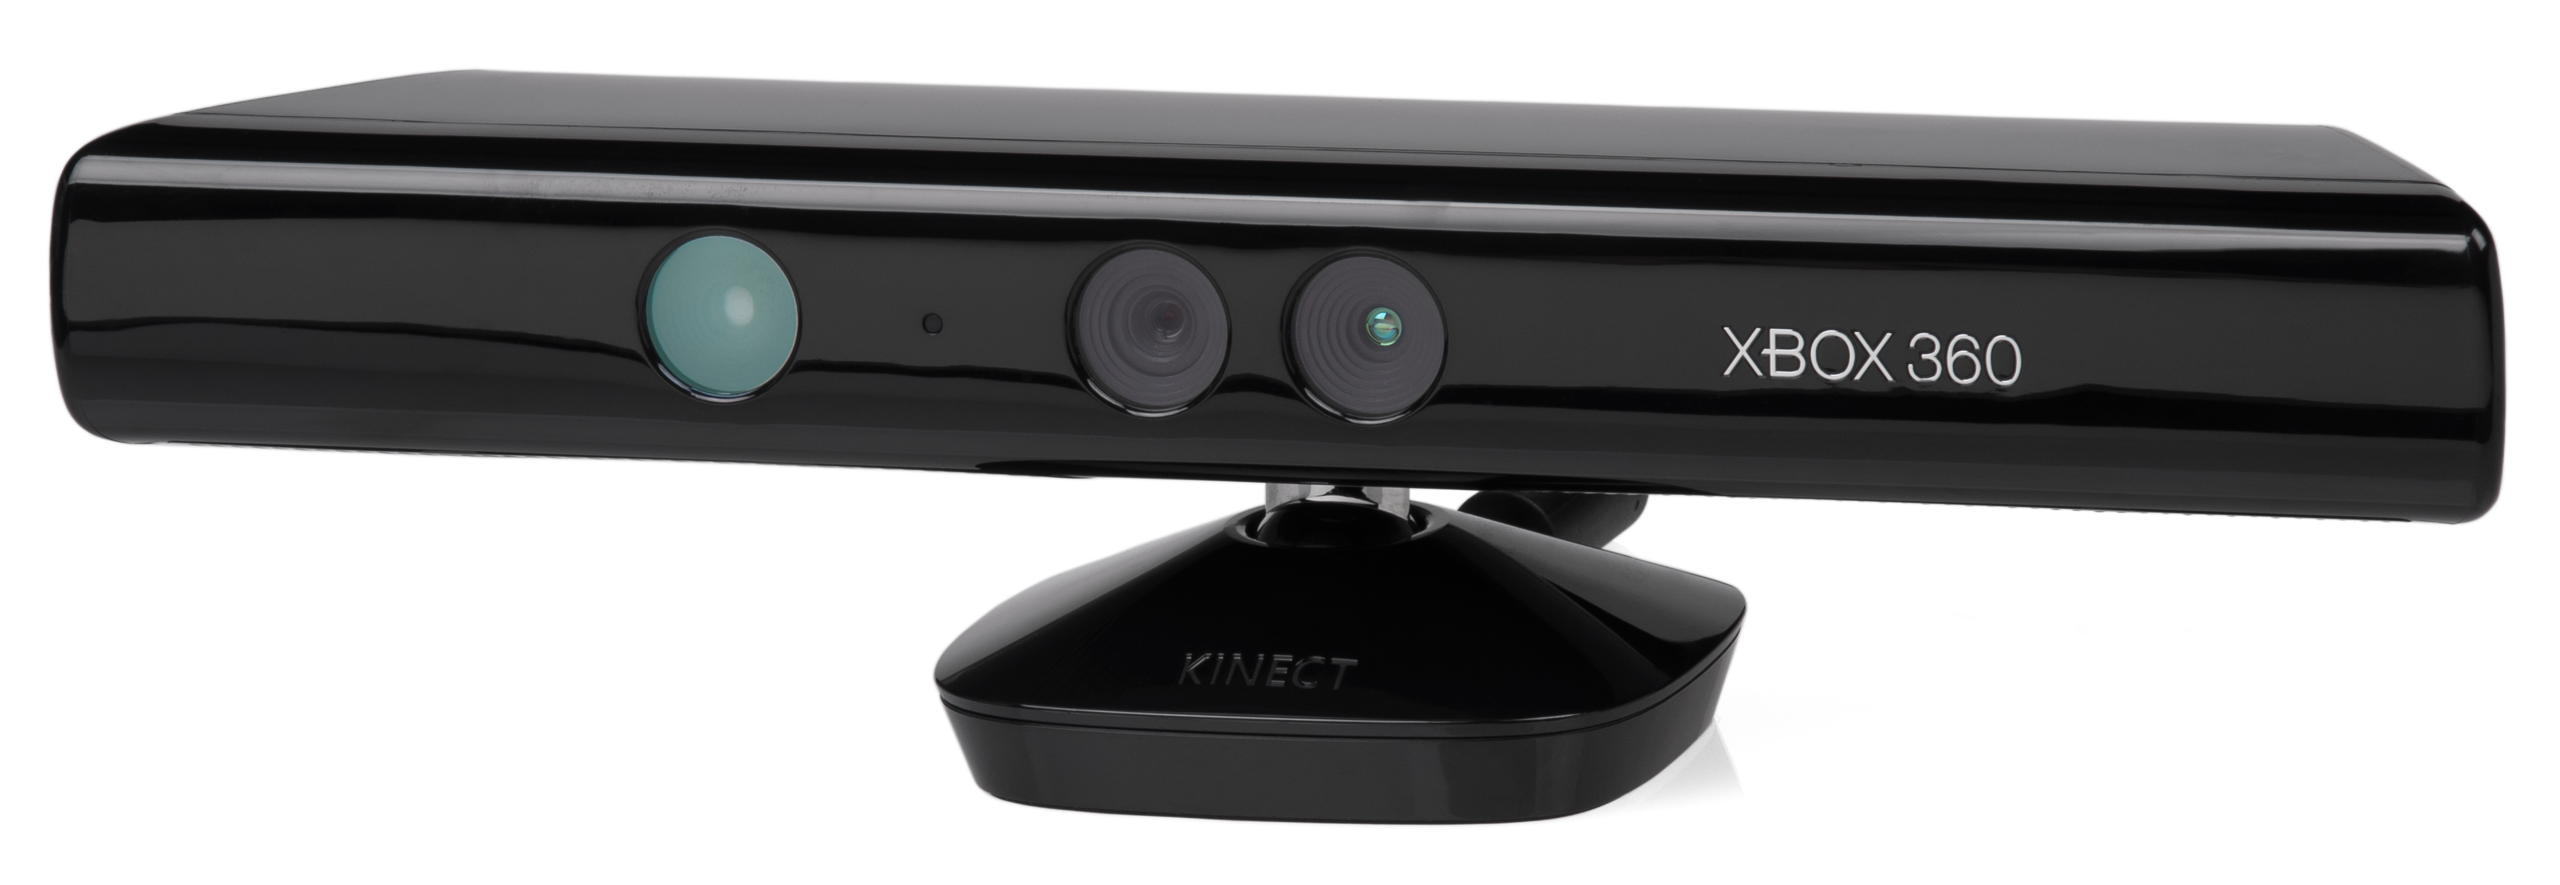
\includegraphics[width=0.45\linewidth]{figs/Xbox-360-Kinect-Standalone.png}(a)
	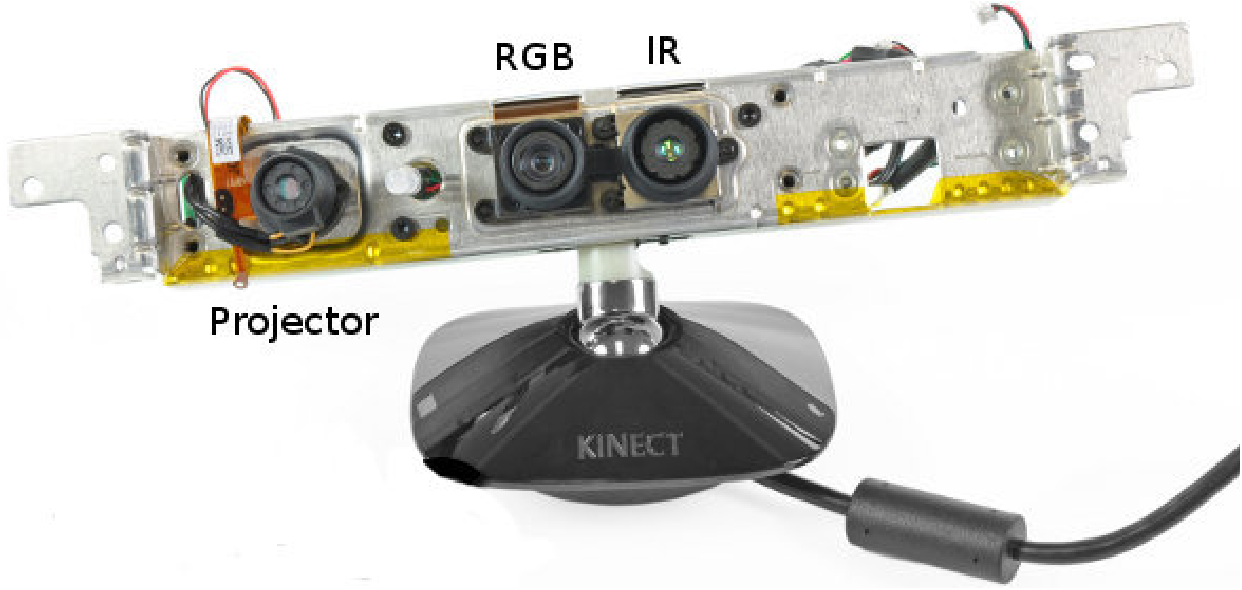
\includegraphics[width=0.45\linewidth]{figs/kinect-internals.pdf}(b)
 	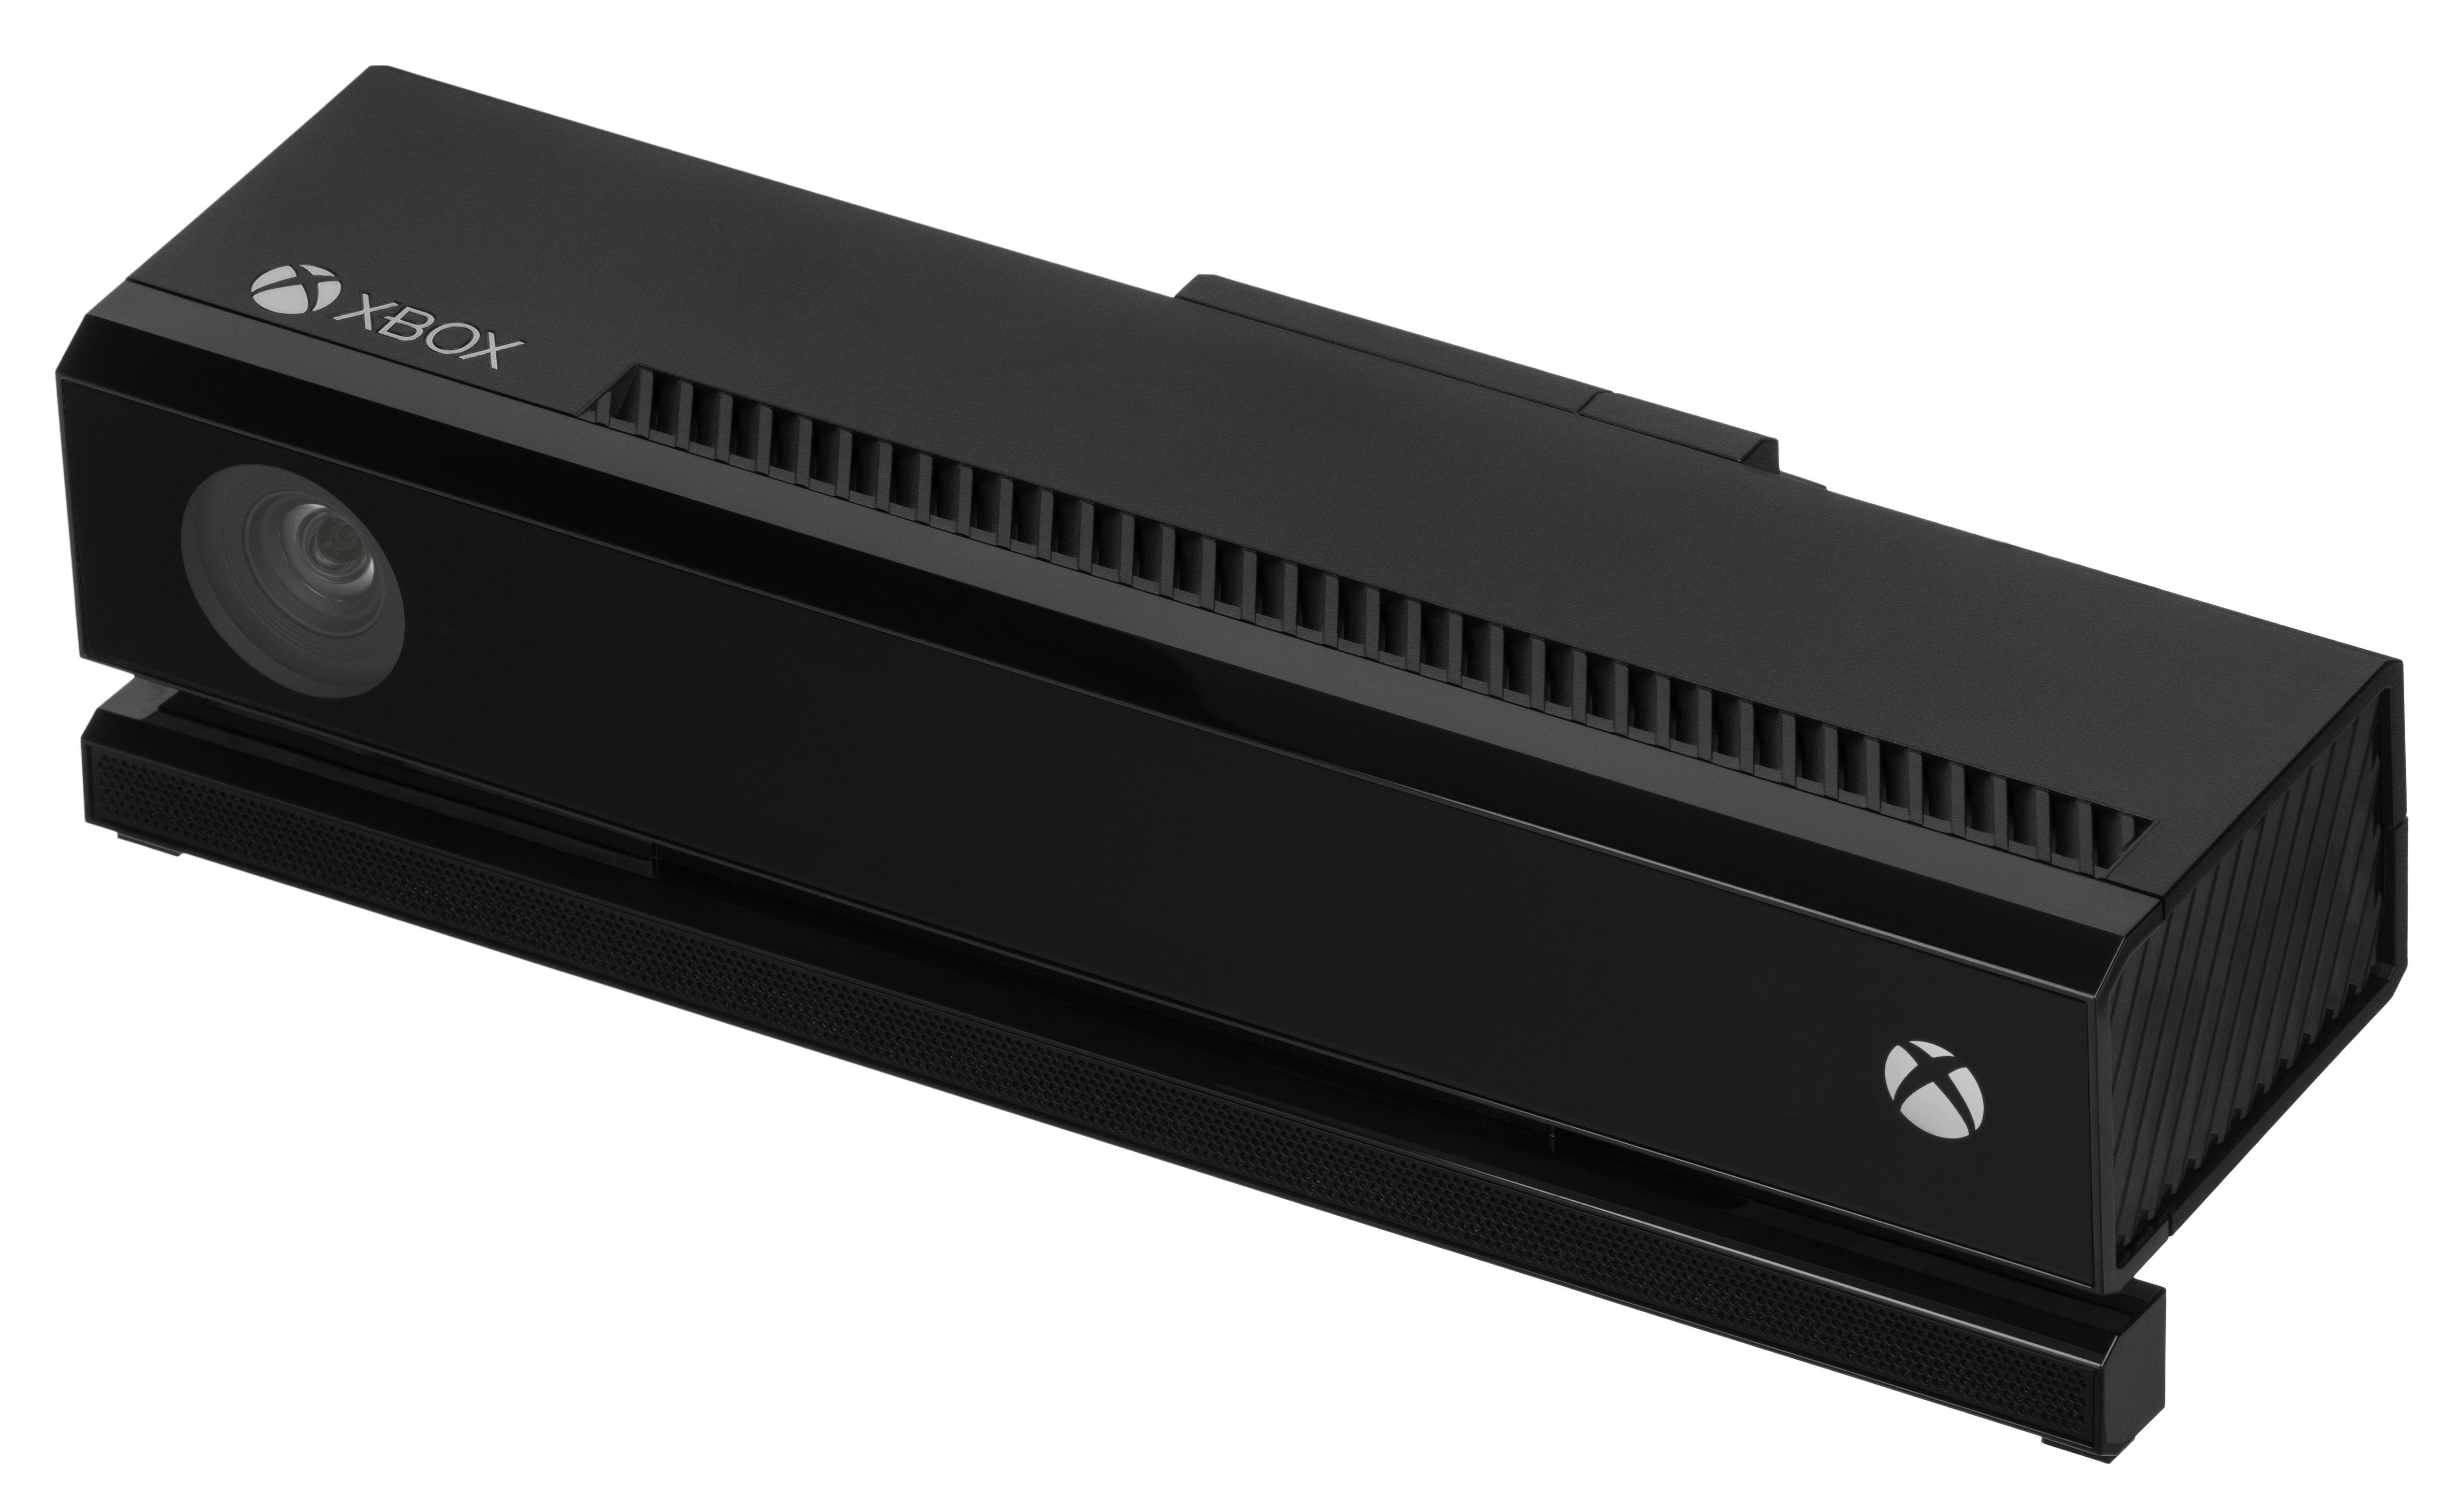
\includegraphics[width=0.45\linewidth]{figs/Xbox-One-Kinect.jpg}(c)
 	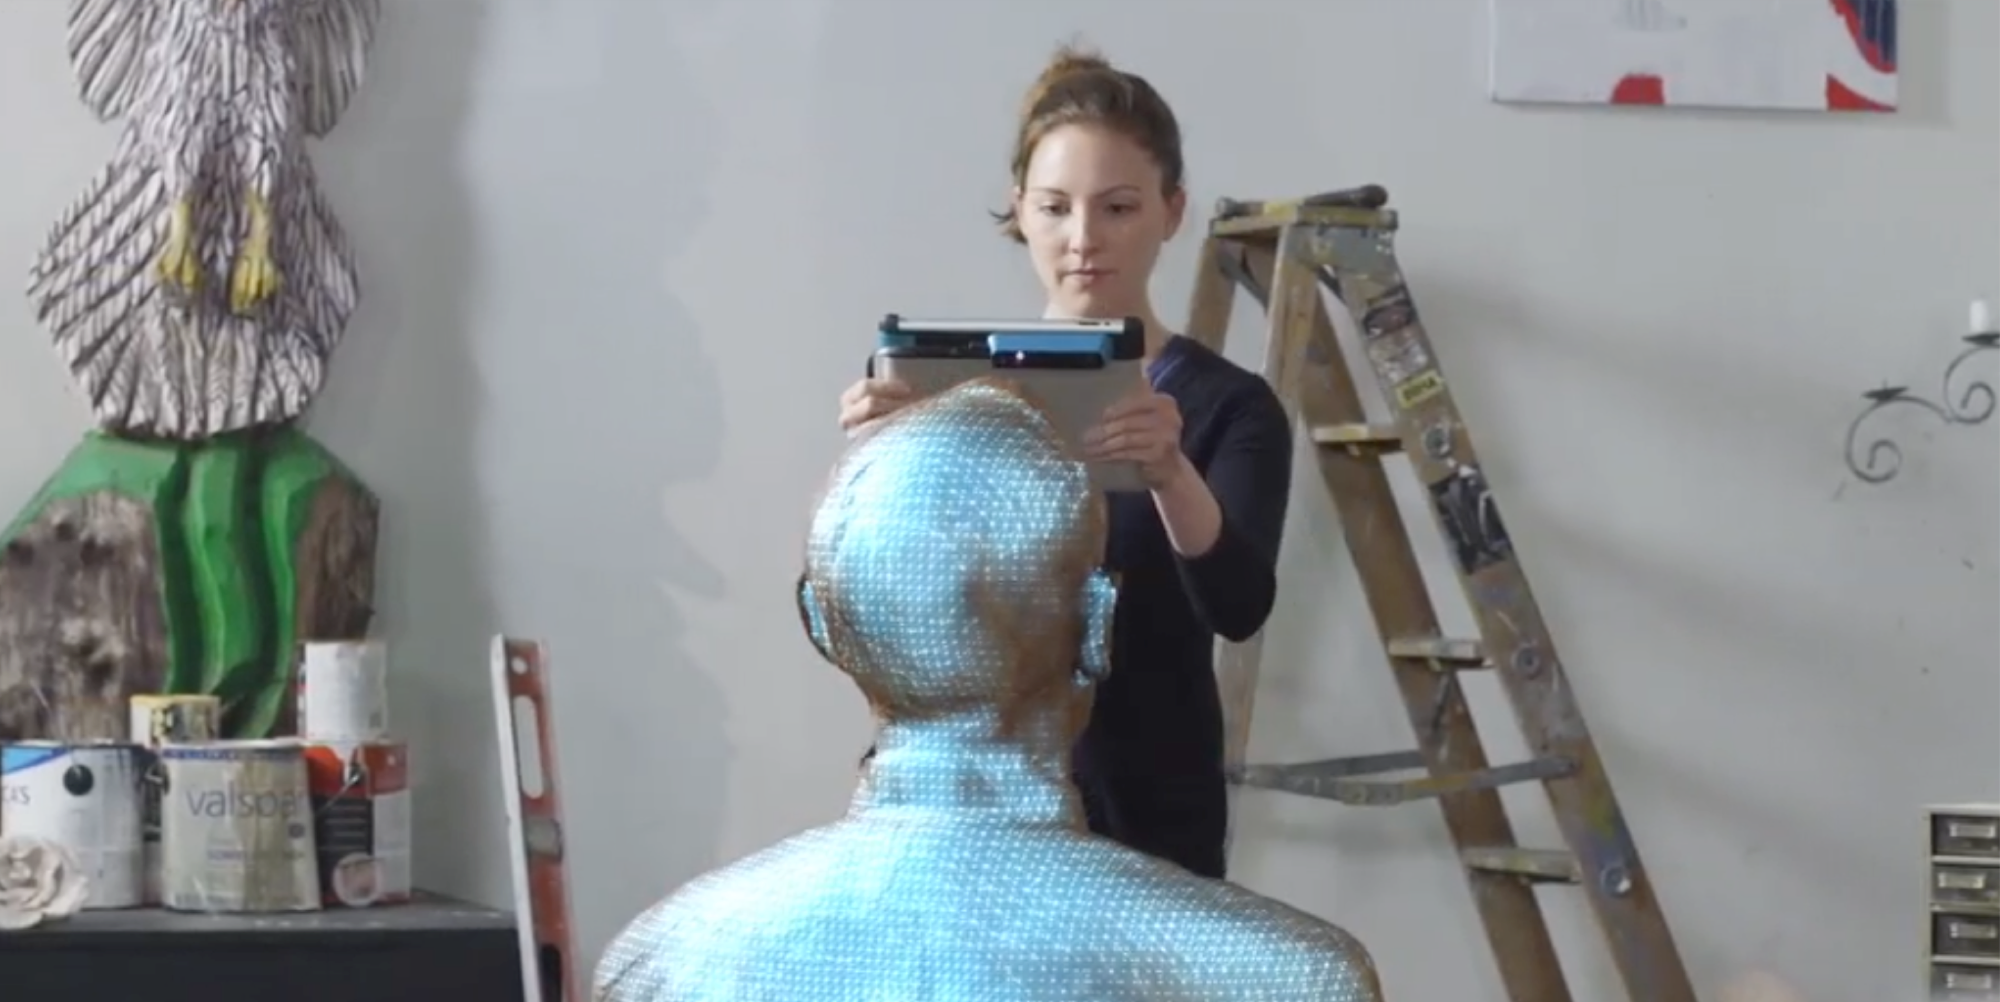
\includegraphics[width=0.45\linewidth]{figs/kinect-handheld1.png} (d)
	\caption{%
   Kinects de primeira geração (a) consistindo de câmeras e projetores
   infra-vermelho (b) e de segunda geração, consistindo de tecnologia ToF (c). 
   Ambos os kinects são largamente utilizados para escaneamento em tempo real, 
   formando a base de escaneadores manuais (d), porém nem sempre são úteis para 
   preservação detalhada de patrimônio. Um dos objetivos deste
   projeto é explorar os limites desta tecnologia.
	}\label{fig:kinect}
\end{figure}

A preservação de patrimônio tem sido realizada tradicionalmente com escaneadores
dedicados de alto custo, como no famoso projeto de escaneamento \emph{in situ} da escultura
David, chamado \emph{Digital Michelangelo}~\cite{levoy2000digital},
Figura~\ref{fig:david}.  O projeto teve início em 1992 e tem como objetivo a
utilização de escaneadores a \emph{laser} de profundidade (\emph{Rangefinder Scanners}),
aliado a algoritmos que combinam diferentes profundidades e cores da imagem,
para realizar uma digitalização da parte externa e da superficie de forma
acurada da estátua de David. Note-se, porém, que esse método pode ser utilizado em diferentes
objetos no mundo real, como partes de máquinas, artefatos culturais e na
indústria de video games, por exemplo.  Para as partes mais detalhadas, foi
utilizado um escaneador de menor escala que faz uma pequena triangulação com
laser de profundidade.

Mais recentemente, pode-se considerar tecnologias mais acessíveis, similares às
de altíssimo custo do projeto Digital Michelangelo e popularizadas na última
década pela indústria de entretenimento, notadamente pelo projeto
Natal/Kinect~\cite{smisek20133d,wang2015research}. A reconstrução usando-se Kinect (de
primeira ou segunda geração) usando software atual de super-resolução, é
inferior à de um sistema a \emph{laser} de alta qualidade, sendo, porém de baixo custo
e muito mais versátil devido ao sistema de aquisição manual e a software
amplamente utilizado e desenvolvido~\cite{wang2015research},
Figura~\ref{fig:rec3d:comparacao}.

% Seria de grande interesse explorar os dois paradigmas supracitados
% para avaliar as possibilidades disponíveis no estado da arte de reconstrução 3D
% para o escaneamento de baixo custo para a preservação de Patrimônio. O que se
% pode atingir com apenas uma filmagem de esculturas realizada por um smartphone,
% sem calibração prévia e \emph{in situ}, ou seja, sem ambiente controlado?  Como
% esta recontrução se compara nos dias de hoje com a reconstrução realizada por um
% escaneador padrão baseado em Kinect?

\begin{figure}[!h]
	\centering
	%   \includegraphics[width=1.0\linewidth]{figs/3d-curve-sketch/system-diagram.eps}
	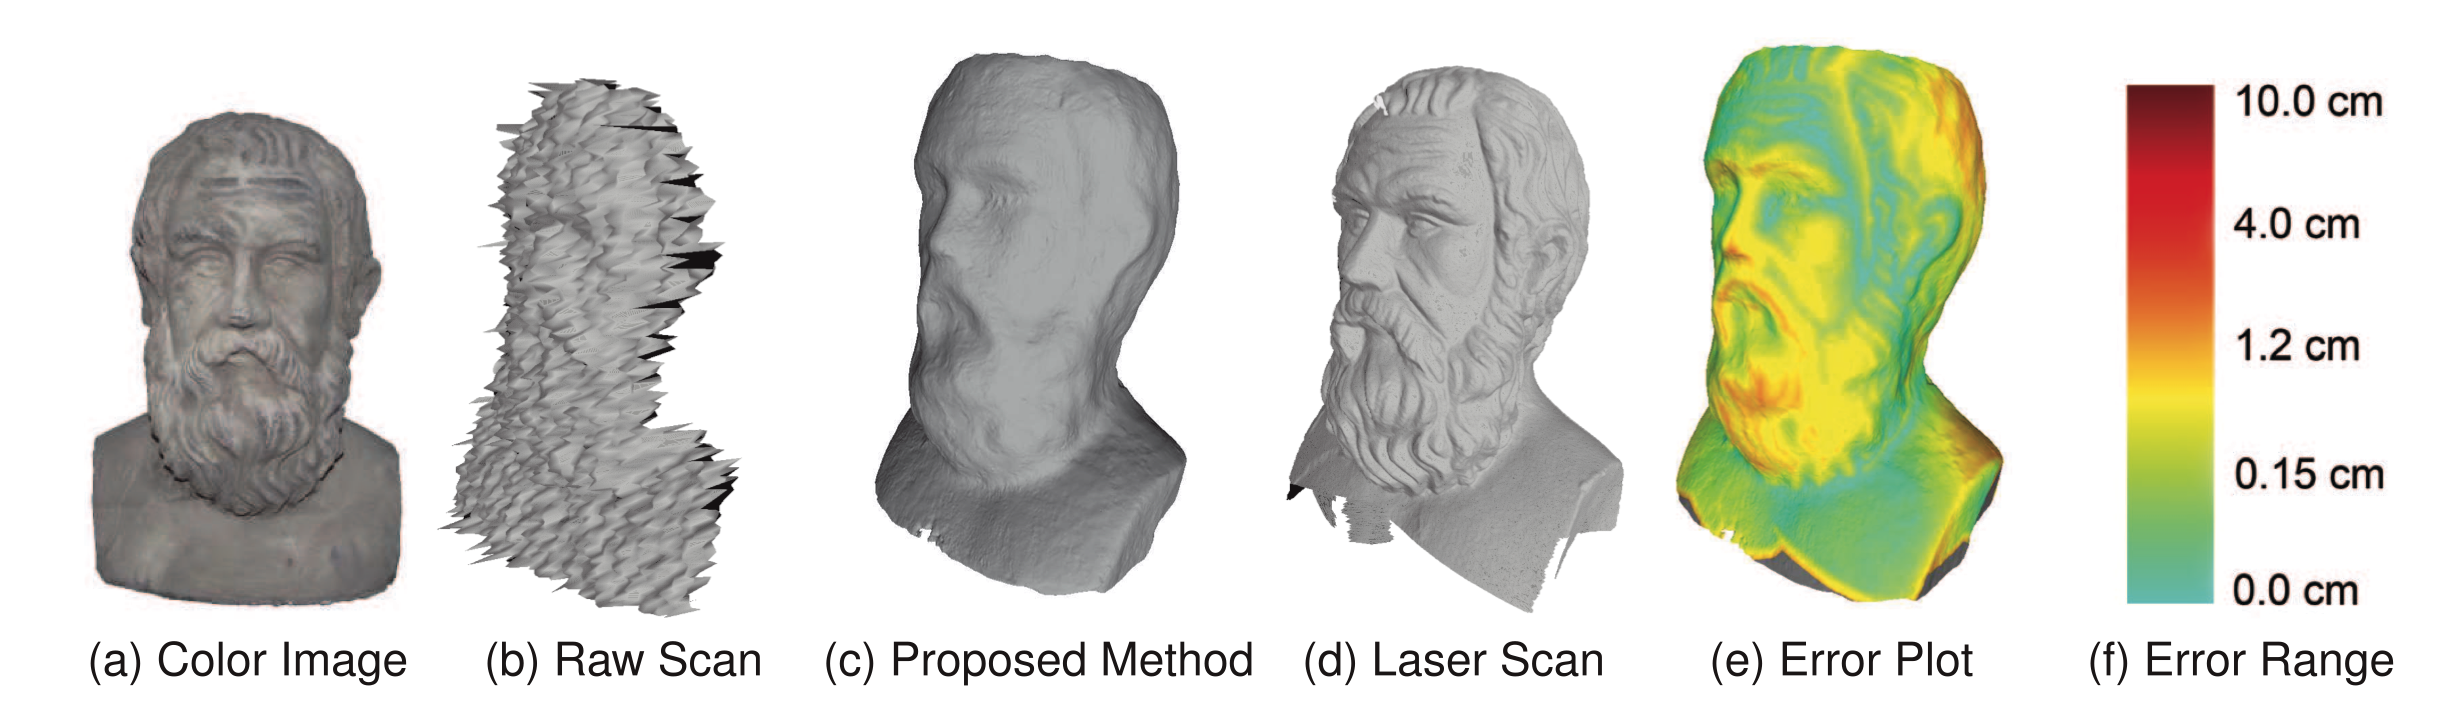
\includegraphics[width=1\linewidth]{figs/kinect-vs-usual.png}
	\caption{%
    A reconstrução usando-se Kinect (de primeira ou segunda geração) usando
    software atual de super-resolução (c) fornece precisão similar a um sistema estéreo de média
    resolução, inferior um sistema a \emph{laser} de alta qualidade (d) porém de baixo custo e
    muito mais versátil~\cite{wang2015research}.
	}\label{fig:rec3d:comparacao}
\end{figure}

\begin{figure}[!h]

\centering

\subfloat[]{\label{fig:davida}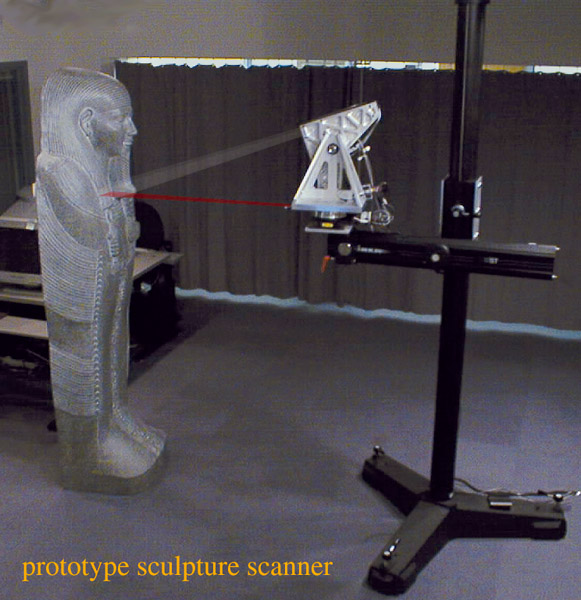
\includegraphics[height=0.38\linewidth]{figs/Proto+Inka+Egypt_light-s.jpg}}
% \vspace{2ex}
\subfloat[]{\label{fig:davidb}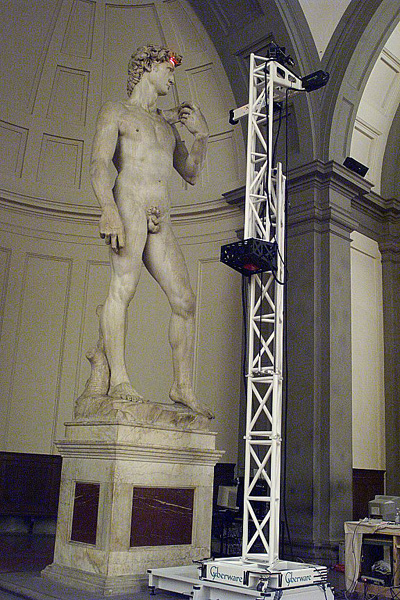
\includegraphics[height=0.38\linewidth]{figs/gantry-with-david-s.jpg}}\\
\subfloat[]{\label{fig:davidc}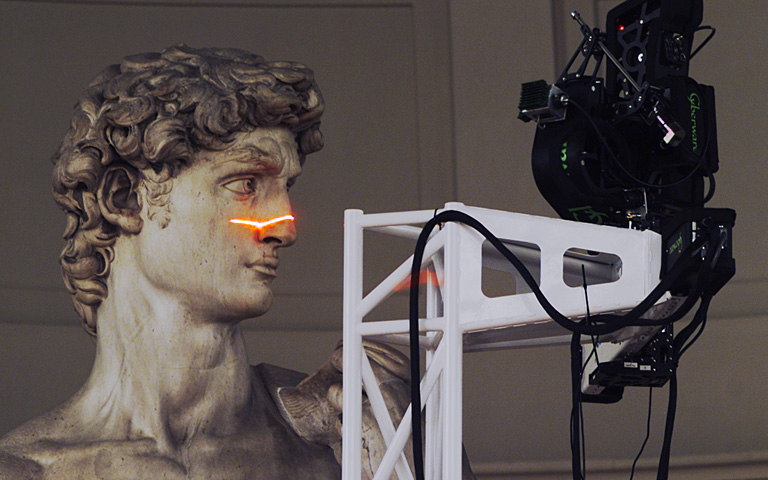
\includegraphics[height=0.25\linewidth]{figs/scanner-head-and-david-head-s.jpg}}
% \vspace{2ex}
\subfloat[]{\label{fig:davidd}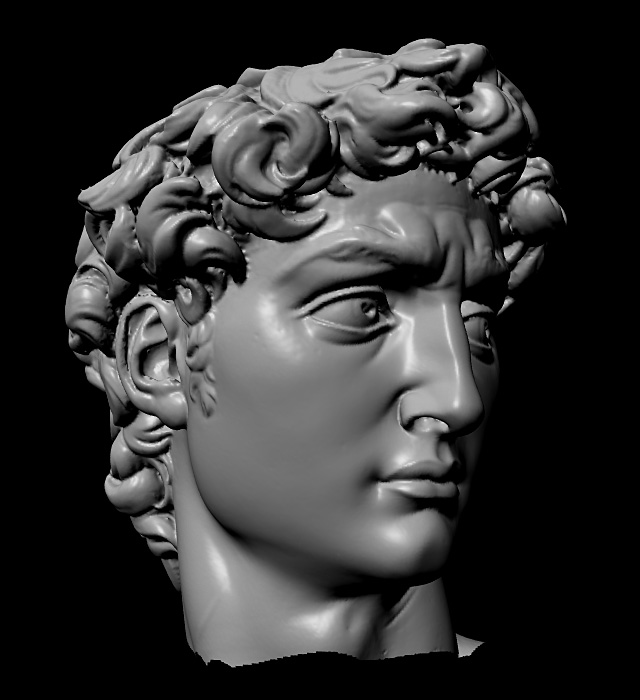
\includegraphics[height=0.25\linewidth]{figs/david-classic-leftlight-s.jpg}}
\caption{%
  Protótipo do escaneador a \emph{laser} do projeto clássico~\emph{Digital
  Michaelangelo}. Em (a), um objeto típico escaneado por um sistema inicial foi uma réplica em tamanho real
   de um sarcófago egípcio. O escaneador foi reconfigurado para objetos maiores, pois 
   a escultura David possui 517 centímetros (b); tabém foi reconfigurado para a cabeça,  
   para girar em 90 graus, que faz o \emph{laser}
   rotacionar da posição horizontal para a vertical e em torno da
   cabeça como um todo (c). Cerca de 100 \emph{scans}
   diversas posições foram alinhados automaticamente por um algoritmo 
   ICP (\emph{iterated-closest-points}). Após uma otimização global para minimizar erros 
   de alinhamento toda a estátua, usa-se um algoritmo VRIP (\emph {volumetric
   range image processing}) (d)~\cite{levoy2000digital}}.
  \label{fig:david}
\end{figure}

\subsection*{O Jardim do Nêgo, Nova Friburgo}
no caso de Nova Friburgo, há a necessidade redobrada de preservação de
patrimônio a céu aberto, em especial devido às chuvas e deslizamentos inerentes à região.  o
jardim do nêgo consiste em grandes esculturas em encostas, cobertas por um tapete de
vegetação, as quais desfrutam de grande reconhecimento regional e internacional~\cite{jardimdonego:theguardian},
Figura~\ref{fig:esculturas}.

\begin{figure} [!h]
	\centering
	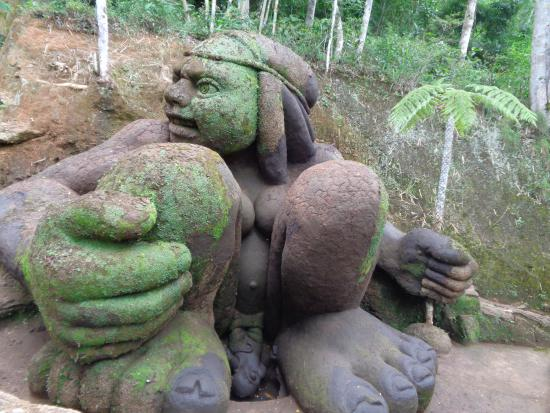
\includegraphics[height=0.23\linewidth]{figs/jardim-do-nego.jpg}
	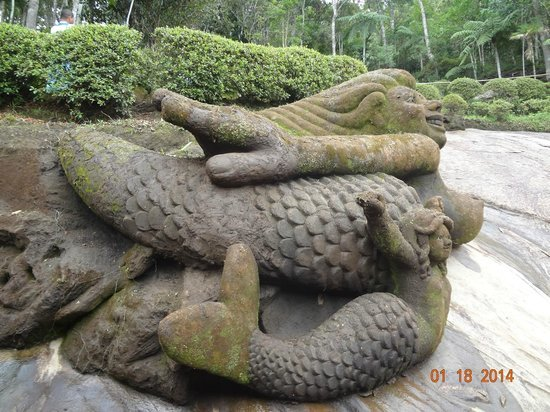
\includegraphics[height=0.23\linewidth]{figs/jardim-do-nego22.jpg}
	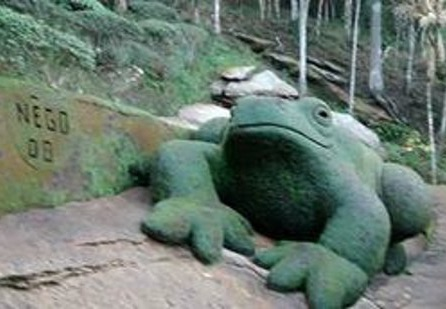
\includegraphics[height=0.23\linewidth]{figs/jardim-do-nego32-small.jpg}
	\caption{Algumas esculturas do Jardim do Nêgo~\cite{JardimDoNego:TheGuardian}}\label{fig:esculturas}
\end{figure}


% \begin{figure} [!h]
% 	\centering
% 	%   \includegraphics[width=1.0\linewidth]{figs/3d-curve-sketch/system-diagram.eps}
% 	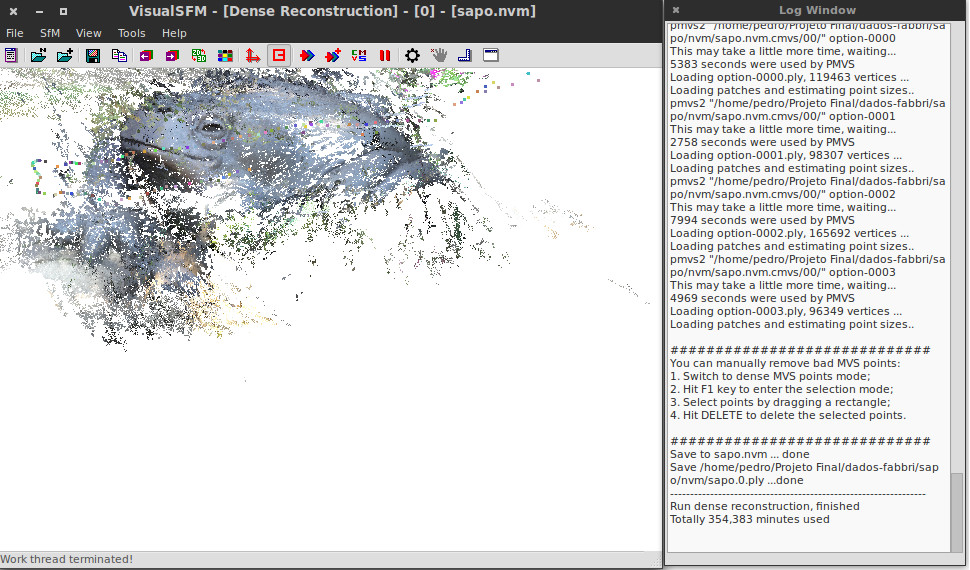
\includegraphics[width=1\linewidth]{figs/rec3d.jpg}
% %	\includegraphics[width=0.95\linewidth]{figs/rec3d-curves-pmvs.pdf}
% 	\label{fig:rec3d}
% 	\caption{A reconstrução usando-se apenas imagens, sem controle de aquisição, 
% 	   como em um vídeo de um smartphone filmado em torno do objeto, fornece uma
% 	   nuvem de pontos, que pode ser
% 	   densificada~\cite{snavely2010bundler,wu2011visualsfm,furukawa2007dense,mve}, ou
% 	   atribuída de
% 	   curvas~\cite{Usumezbas:Fabbri:Kimia:ECCV16,Fabbri:Kimia:IJCV2016,Fabbri:Kimia:CVPR10,Fabbri:Giblin:Kimia:ECCV12}, de forma a preservar a resolução
% 	   em áreas de alto conteúdo informativo. Tais representações estão sendo
% 	   atualmente unificadas na pesquisa da área. Este projeto propõe explorar os
% 	   limites da reconstrução 3D usando-se apenas imagens, no contexto de
% 	   preservação de patrimônio.}
% \end{figure}


Idealizado e criado por Geraldo Simplicio (Nêgo), artista cearense que mora no
local a mais de 30 anos, e que ganhou notoriedade por suas esculturas de barro,
com traços singulares e técnicas únicas. Hoje, trabalha para reconstruir o
Jardim após a tragédia de 2011 na região serrana, onde algumas estruturas foram
destruídas. Portanto, com o consentimento do Nêgo, surgiu a motivação desta
pesquisa: além de explorar métodos de reconstrução, também tem o objetivo de
ajudar a criar sistemas completos para eternizar um patrimônio que é reconhecido
no mundo todo.

A preservação das esculturas do Jardim do Nêgo se mostra um desafio à pesquisa em
recontrução 3D, pois apresentam curvas bem delineadas, que são 
representadas de maneira suavizada e empobrecida por métodos convencionais.
Algumas esculturas apresentam pouca textura, com apenas um leve padrão de musgo.
Seria de grande interesse avaliar o potencial de técnicas atuais de
reconstrução 3D geral que não exigem controle preciso de aquisição, as quais têm seu código fonte
disponível na internet.

\newpage

\section{Objetivos}\label{sec:objetivos}

Pretende-se, ao longo deste projeto, ganhar experiência com técnicas
modernas de reconstrução 3D fotogramétrica, no contexto de uma aplicação
bem-definida de preservação de patrimônio. 
% A entrada do sistema deverá ser um
% conjunto de vídeos realizados por câmeras de baixo custo, ou um conjunto de
% escaneamentos realizados por escaneadores à mão de baixo custo baseados em Kinect.

O objetivo concreto é explorar as tecnologias supracitadas para
desenvolver um esquema de escaneamento de patrimônio usando software aberto, câmeras e
escaneadores de baixo custo, representando o estado da arte em reconstrução 3D sem
restrições de aquisição. Perguntas fundamentais a serem respondidas são: que
nível de detalhe, facilidade e precisão se pode obter usando-se apenas imagens e software
aberto? É possível utilizar escaneadores de baixo custo baseados em Kinect com
melhorias significativas em termos de qualidade, conveniência ou tempo de
processamento?  Quais são as restrições desses sistemas? Seria útil, na prática,
uma reconstrução de curvas para auxiliar na reconstrução de nuvem de pontos e de
superfícies densas? Onde o estado da arte deve ser avançado de forma a permitir
uma solução mais conveniente e completa para a preservação de patrimônio?

O principal objetivo em termos de pesquisa científica será comparar as
diferentes abordagens do estado da arte disponíveis para reconstrução 3D e
explicitar suas limitações práticas.

\section*{Organização deste manuscrito}

Este trabalho foi estruturado da seguinte maneira: Introduzimos
métodos baseados em reconstrução a \emph{laser} no Capítulo~\ref{cap:laser},
apresentando, de uma maneira mais técnica, o projeto \emph{Digital
Michelangelo} na Seção~\ref{sec:David}, que foi um dos pioneiros na técnica de
conservação de acervos culturais. No próximo Capítulo~\ref{cap:kinect},
discutimos o uso do Kinect, da Microsoft, no que tange à calibração do sistema
para o uso em tecnologias \emph{Structure from Motion}.  Adiante, no
Capítulo~\ref{cap:pontosdeinteresse}, abordaremos o tema central do trabalho:
técnicas de reconstrução baseadas em fotogrametria, com o emprego de dois
softwares, o MVE~\ref{sec:mve} e o VisualSfM~\ref{sec:visualsfm} e seus
respectivos funcionamentos. Ao final, apresentamos experimentos e conclusões
do trabalho, bem como sugestões para implementações e trabalhos futuros.

% O trabalho foi estruturado da seguinte maneira: previamente introduzimos os métodos baseados em pontos de interesse no Capítulo~\ref{sec:pontosdeinteresse}, destacando suas funcionalidades. No Capítulo~\ref{sec:denserecon} discutimos e aprofundamos o  funcionamento de cada algoritmo de reconstrução densa empregados, apresentando e debatendo, comparativamente, pontos à favor e contra; O Capítulo~\ref{sec:kinect} é apresentada a técnica de reconstrução utilizada nos  {\it Kinects}, da Microsoft; Com isso, temos o  Capítulo~\ref{sec:visualsfm}, que é dedicado à ferramenta gráfica utilizada para a obtenção dos resultados (VisualSfM) dos algoritmos de reconstrução densa utilizados. Finalmente, apresentamos os resultados e conclusões do trabalho, bem como sugestões para implementações e trabalhos futuros.
%Este trabalho está organizado da seguinte forma: discutimos as técnicas de
%extração de curva sem aprendizagem de máquina supervisionada no
%Capítulo~\ref{sec:cfrag:extraction}. No Capítulo~\ref{sec:learning:chapter},
%discutimos maneiras pelas quais essas técnicas podem ser melhoradas
%usando dados de treinamento anotados por humanos como entrada para uma
%aprendizagem de máquina geométrica de topologia e semântica de fragmentos de
%curva. A maior parte deste material é
%de~\cite{Guo:etal:CVPR14,Guo:etal:PAMI2017:submitted,Tamrakar:PHD:2008}, com esclarecimentos
%substanciais e comentários sobre as questões relativas aos nossos objetivos
%específicos. No Capítulo~\ref{sec:generic:datasets}, apresentamos o processo de
%captura de dados confiáveis (\emph{ground-truth}), comparando os conjuntos de dados anteriores com o problema proposto
%neste trabalho para a água. Nos capítulos restantes, apresentamos e discutimos
%nossos resultados para vários vídeos em tanques de água. Partes deste trabalho
%foram apresentadas em~\cite{Fabbri:WaterWaves2016,Fabbri:WaterWaves2017,Souza:Fabbri:WaterWaves2017}.

%======================================================================================

\chapter*{Reconstrução à Laser}\label{sec:laser}

\section{Introdução}

A técnica de reconstrução baseada em laser é conhecida desde o século passado, pois oferecem uma alta qualidade geométrica de dados, os resultados são em tempo real e requer pouco tempo de captura de dados. 

\begin{figure}[!h]
	\centering
	%   \includegraphics[width=1.0\linewidth]{figs/3d-curve-sketch/system-diagram.eps}
	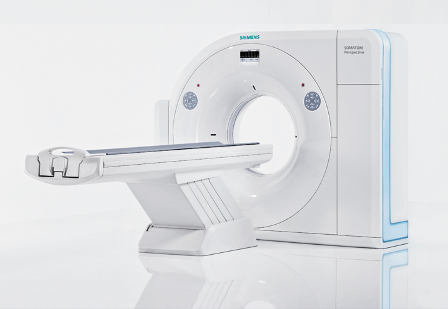
\includegraphics[width=1\linewidth]{figs/tomografia.png}
	\caption{%
	Exemplo de reconstrução à laser utilizando o método baseado em volume.
	%\cite{Cui:Theobalt:etal:PAMI2013,Pajdla:etal:ICCV2011}.
	}\label{fig:laservolume}
\end{figure}

Existem alguns tipos de reconstruções empregando lasers, baseados em volume (ressonância, tomografia, por exemplo \ref{fig:laservolume} ou em superfície (estereoscopia, {\it time of flight}, luz estruturada) . Neste caso, abordaremos o projeto de escaneamento da escultura de Michelangelo, David, que utiliza escaners baseados em superfícies, mais especificamente, utilizando luz estruturada.

\section{Projeto de preservação das esculturas de Michelangelo}

Este projeto tem como motivação avançar a tecnologia de digitalização 3D e criar um acervo digital sobre alguns dos principais artefatos culturais. Foi utilizada uma tecnologia chamada de {\it rangefinder}, com uma equipe de mais de 30 professores, funcionários e estudantes da Universidade de Stanford desenvolveram algoritmos para combinar imagens de múltiplas gamas e cores, passaram os anos de 1998 e 1999 na Itália escaneando esclturas de Michelangelo. 

Pipeline:

O principal componente de {\it hardware} do sistema é um escaner de triangulação à laser, que é composto por 4 eixos motorizados, utiliza um laser, uma câmera de alcance, uma câmera de cores e uma luz branca, isso tudo acrescido de estruturas para estátuas grandes. O objetivo de um escaner deste porte era capturar marcas menores que um milímetro, das ferramentas utilizadas por Michelangelo em suas esculturas. 
Para isso foram testadas diversas resoluções, na qual foi decidido um espaçamento Y (ao longo da faixa do laser) de 1/4 mm e uma resolução Z (profundidade) de pelo menos duas vezes este valor. O que resultou em uma visualização de 14 cm de largura (ao longo da faixa do laser) por 14 cm de profundidade. Caso esta resolução fosse menor, as marcas de cinzelão ficariam borradas e se fosse maior, o conjunto de dados produzido seria gigantesco.
Felizmente, a maioria das estátuas feitas por Michelangelo foram esculpidas com um mármore encontrado em Carrara Statuario, uma pedra altamente uniforme, não direcional e constituída de grãos finos. Além disso, com exceção da "Noite", as esculturas não são polidas e cobertas por terra, o que aumenta a dispersão superficial e reduz a abaixo da superfície.
Neste contexto, a dispersão abaixo da superfície causa alguns problemas: não se pode assumir que a superfície é Lambertiana ideal (%CITAR LAMBERTIANO AQUI%
), mudou a forma com que a renderização dos modelos seriam feitos e diminuiu a qualidade de disposição de dados.
Calibração:
O objetivo de calibrar o aparato era encontrar um mapeamento de coordenadas 2D no seu alcance e cores para coordenadas 3D em um quadro de referência global. Idealmente, este quadro deve ser a estátua (estacionária). Porém não foi rastreado o aparato, ele tornou-se a própria referência. O mapeamento final foi realizado alinhando novas varreduras, com varreduras previamente existentes.
Para calibrar qualquer sistema, primeiramente escolhe-se um modelo matemático que se aproxime do comportamento do sistema, então estima-se parâmetros desse modelo medindo o comportamento do sistema. No caso do projeto de David, o modelo matemático natural era um modelo geométrico 3D parametrizado da cabeça digitalizada e do aparato. Se os componentes do sistema forem suficientemente independentes, a calibração pode ser dividida em estágios, correspondente a cada componente do sistema. Por isso o aparato foi construído pensando na rigidez (independência), pois particionar a calibração em etapas reduz o grau de liberdade em cada etapa, e com isso, o número de medidas necessárias para calibrar este estágio.
Em um sistema mecânico, também é reduzido o volume físico total na qual essas medidas de calibração devem ser tomadas. Além disso, uma calibração em etapas é menos suscetível a propagação de erros, pois caso uma calibração falhasse, seria apenas uma parte da calibração e não o sistema como um todo. No projeto de David, a calibração foi divida em seis etapas distintas:

\begin{enumerate}
\item{Um mapeamento 2D a partir de coordenadas de {\it pixels} das imagens da câmera para locais físicos na camada de laser}
\item{Transformação rígida 2D/3D do sistema de coordenadas da camada do laser para esferas de aço anexadas ao escaner da cabeça}
\item{Transformação rígida 3D para acomodar o rolamento do escaner da cabeça em 90 $^{circ}$ (ao remontá-lo) em relação ao conjunto de inclinação}
\item{A localização do eixo de rotação de inclinação e o mapeamento não-linear de movimento comandos para ângulos de rotação físicas}
\item{A localização do eixo de rotação panorâmico e o mapeamento de seus comandos de movimento para ângulos de rotação física}
\item{A localização do eixo de translação, que também depende de como o conjunto inclinação-panorâmico está montado no braço horizontal}
\end{enumerate}

O resultado da calibração pode ser descrito como uma concatenação de seis matrizes 4x4:
\[
\begin{bmatrix}
\text{translação} \\ 
\text{horizontal}
\end{bmatrix}
\begin{bmatrix}
\text{rotação} \\ 
\text{panorâmica}
\end{bmatrix}
\begin{bmatrix}
\text{rotação} \\
\text{de} \\
\text{inclinação}
\end{bmatrix}
\begin{bmatrix}
\text{rotação} \\
\text{de} \\
\text{rolamento}
\end{bmatrix}
\begin{bmatrix}
\text{laser para o} \\
\text{escaner }
\text{da cabeça}
\end{bmatrix}
\begin{bmatrix}
\text{imagem} \\
\text{para o} \\
\text{laser}
\end{bmatrix}
\]
%  \] \[  \] \[  \] \[ \text{rotação de rolamento} \] \[ \text{laser para o escaner da cabeça} \] \[ \text{imagem para o laser} 
%\end{gather*}

Calibração do sistema de cores:
Para corrigir a distorção geométrica na câmera de cores, foi fotografado um alvo de calibração planar que possui um certo número de {\it features} que, por sua vez, foram usados para calcular os parâmetros intrínsecos da câmera. Estão inclusos no modelo dois termos de distorção radial e dois termos de distorção tangencial que tem uma projeção de perspectiva fora do centro e uma escala possivelmente não uniforme (em X e Y) %CITAR[Heikkila..97].%

Para obter um mapeamento da câmera colorida para o escaner da cabeça, o alvo foi escaneado usando o laser e a câmera de alcance. Uma vez que o escaner retornou a intensidade refletida pelo laser, bem como a profundidade, pode-se calcular as coordenadas 3D de cada ponto da {\it feature}.

Para corrigir os efeitos radiométricos espaciais, incluindo o aspecto de vinheta das lentes, a não uniformidade angular, o declínio da lei quadrada inversa dos holofotes e a não uniformidade espacial na resposta do sensor, foi fotografado um cartão branco sob o holofote e construída uma tabela de correção de intensidade por pixel.
% Depois de testar várias resoluções, decidimos um espaçamento de amostra Y (ao longo da faixa laser) de 1/4 mm e uma resolução Z (profundidade) pelo menos duas vezes esta multa 1. Isso nos deu uma visão de 14 cm de largura (ao longo da faixa a laser ) por 14 cm de profundidade. Em retrospectiva, ficamos satisfeitos com a resolução que escolhemos; Qualquer coisa menor teria significativamente borrado as marcas de cinzelão de Michelangelo, e qualquer coisa maior teria tornado os nossos conjuntos de dados não gerenciáveis.

%FIGURA DAS FERRAMENTAS AQUI%

Procedimento de digitalização:
Passos para digitalização: Um operador move, interativamente o escaner da cabeça através de uma sequencia de movimentos, definindo os limites de volume a ser escaneado. O volume que pode ser coberto em uma única varredura, foi delimitado por conta de quatro fatores:
\begin{itemize}
\item{O campo de visão e os limites de movimento do escaner}
\item{A  queda na qualidade da varredura com o aumento da obliquidade do laser}
\item{Oclusões, tanto do laser quanto da linha de visão da câmera}
\item{Obstruções físicas, como paredes, estátuas ou o próprio equipamento}
\end{itemize}

Uma vez planejada a varredura, um script de digitalização é executado automaticamente, levando desde alguns minutos, até horas para terminar, dependendo da largura da área a ser coberta.


% Range scanning. A typical range scan consisted of several con-
% centric curved shells separated by translational motion of the scan
% head along the horizontal table. Each shell in turn consisted of sev-
% eral horizontally adjacent vertical sweeps of the laser, as shown in
% figure 5. If the laser line was turned vertically, then the sweeps were
% horizontal instead. We decided to overlap adjacent sweeps and
% shells by 40% and 15%, respectively - enough to align them in soft-
% ware in the absence of precisely calibrated motion. Since scanning
% was slow (1 cm per second), we preceded each sweep with a high-
% speed (10 cm per second), low-resolution pre-scan that conserva-
% tively determined which part of the sweep actually contained data.

%Alcance da varredura
Alcance da varredura
% Escala de varredura. Uma varredura de varredura típica consistiu em vários reservatórios curvos concêntricos separados pelo movimento de translação da cabeça de varredura ao longo da mesa horizontal. Cada casca, por sua vez, consistiu em vários varredões verticais horizontais adjacentes do laser, como mostrado na figura 5. Se a linha do laser foi girada verticalmente, então os varreduras estavam em vez da horizontal. Decidimos sobrepor as varreduras e os reservatórios adjacentes em 40% e 15%, respectivamente - o suficiente para alinhá-los no software na ausência de movimento calibrado com precisão. Uma vez que a varredura foi lenta (1 cm por segundo), precedemos cada varredura com uma pré-digitalização de alta velocidade (10 cm por segundo) e de baixa resolução que determinou de forma conservadora qual parte da varredura realmente continha dados.

% O principal componente de hardware do nosso sistema foi um scanner de triangulação a laser e um pórtico motorizado personalizado para digitalizar grandes estátuas. Nossos requisitos para este scanner eram exigentes; queríamos capturar marcas de cinzelão menores do que um milímetro, queríamos capturá-las a uma distância segura, e queríamos chegar ao topo do David de Michelangelo, que tem 23 pés de altura no pedestal. Nas seções que se seguem, descrevemos os sistemas de aquisição de alcance e cor deste scanner, seu pórtico mecânico de suporte e nosso procedimento para calibrá-lo.

Primeiramente faz-se o escaneamento da geometria da escultura:
\begin{itemize}
\item{Alinhamento manual}
\item{ICP -- {\it Iterative Closest Point} para uma câmera existente} %CITAR ICP AQUI%
\item{ICP automático para todos os pares sobrepostos}
\item{Relaxação global para espalhar o erro}
\item{Reunir utilizando métodos volumétricos}
\end{itemize}


Após isso, ocorre o escaneamento e processamento das cores da escultura:

\begin{itemize}
\item{Compensação da iluminação do ambiente}
\item{Descarte de pixels com sombra ou especulares}
\item{Mapeia-se os vértices (uma cor por vértice)}
\item{Correção da irradiância e reflectância difusa}
\end{itemize}

Limitações:
\begin{itemize}
\item{Inter-reflexões são ignoradas}
\item{Dispersões subterrâneas são ignoradas}
\item{Tratamento difuso com Lambertiano} %CITAR TREATED DIFFUSED AS LAMBERTIAN%
\item{Usa superfícies normais agregadas}
\end{itemize}

O projeto não teve mais nenhum avanço desde o verão de 2004, por falta de financiamento. Como resultado, modelos de alta qualidade só existem do David na resolução de 1,0 mm (56 milhões de triângulos) e São Mateus a 0,25 mm (372 milhões de triângulos). Um modelo também existe para o Atlas em 0,25 mm (aproximadamente 500 milhões de triângulos), mas contém erros de alinhamento. Após 6 anos de trabalho estudantil remunerado e voluntário, existem modelos para cada um dos 1.186 fragmentos. Esses modelos, que totalizam quase 8 bilhões de polígonos, se encontram no próprio site da Universidade de Stanford %CITAR AQUI$. 

Também foram disponibilizadas algumas métricas sobre este projeto \ref{tab:metricasDavid}.

\begin{table}
\caption{Métricas do projeto de reconstrução da escultura David}
\label{tab:metricasDavid}
\begin{tabular}{|l|p{4.7cm}|}
\hline
Números de objetos escaneados          & 10 estátuas + 2 edificações + 1,163 fragmentos de mapa  \\ \hline
Menor e maior objetos escaneados       & 1 polegada (fragmentos de mapa) e 23 pés (David)         \\ \hline
Resolução espacial dos dados                & 0.29mm para geometria, 0.125mm para cor              \\ \hline
Complexidade do maior conjunto de dados             & 2 bilhões de polígonos + 7,000 imagens (David)\\ \hline
Tamanho do maior conjunto de dados                    & 32 {\it gigabytes} (David)                  \\ \hline
Quantia total de dados capturados              & 250 {\it gigabytes}                                 \\ \hline
Tamanho do maior escaner                    & 24 pés de altura, 1800 libras de peso                  \\ \hline
Peso total do equipamento levado para a Itália & 4 toneladas                                              \\ \hline
Número de pessoas envolvidas                  & 32 (sem incluir subcontratantes e colaboradores) \\ \hline
Tempo médio para escaneamento              & 1 semana (exceto o David, que levou 1 mês)       \\ \hline
Tempo total de escaneamento                 & 5,000 horas de trabalho                                   \\ \hline
Total de tempo para processamento de dados          & 4,000 horas de trabalho (até agora)                            \\ \hline
Custo do projeto                          & \$2,000,000                                         \\ \hline
\end{tabular}
\end{table}
%COLOCAR FOTOS DAVID%
Porém, devido ao seu alto custo com equipamentos, com {\it softwares} e sem falar na necessidade de estações robustas para armazenamento dos dados e para esacaneamento de patrimônios, outras técnicas foram emergindo com o passar dos anos, como a fotogrametria, que será abordada mais tarde neste documento.

\chapter{Kinect}\label{sec:kinect}
%======================================================================================
Um componente criado pela Microsoft para fins recreativos (como no XBox, por exemplo), virou uma das mais conhecidas ferramentas de reconstrução 3D no cenário atual. Sua primeira versão (Kinect V1) utiliza uma técnica similar à empregada no projeto da Universidade de Stanford, com luz estruturada, porém, diferentemente dos escaners à laser, o Kinect tem um custo monetário baixo e é acessível a todo público em geral (desde entusiastas, amadores até profissionais da área). 

O Kinect V2 utiliza uma projeção de fótons [...] e por isso ele já não é tão utilizado na área de reconstrução 3D como o V1. 

O V1 é composto por 2 câmeras: uma RGB e outra de profundidade e por um projetor IR ({\it infra-red}) de padrões. E funciona da seguinte maneira: o projetor IR de padrões lança uma matriz que é conhecida pelo Kinect, a partir disso, qualquer deformação deste padrão é captada pelas câmeras, o que identifica se um objeto está no alcance dos sensores ou não. A resposta, é composta por 3 {\it outputs}: uma imagem IR,  uma RGB e a profundidade (inversa) da imagem.

%IMAGEM KINECT%

Sua principal saída da imagem do Kinect é correspondente à profundidade da cena. Em vez de providenciar uma profundidade {\it Z}, ele retorna uma profundidade inversa, {\it D}.
A profundidade da imagem é construída a partir da triangulação da imagem IR com o projetor e, consequentemente, "carregada" pela imagem IR.

%IMAGEM PROFUNDIDADE KINECT%
 
Foram realizados alguns experimentos associando fotogrametria com o Kinect V1. Primeiramente, foi executado uma calibração do Kinect para este tipo de reconstrução, onde a partir de experimentos, o sistema foi modelado como \ref{eq:kinectCalibracao}.

\begin{equation}
\label{eq:kinectCalibracao}
q(z)=2.73z^{2}+0.74z 0.58
\end{equation}

Onde "z" é a profundidade em metros, e "q" a quantização.

O modelo geométrico do kinect foi criado com um sistema multi-view considerando o RGB, IR e a profundidade
\begin{gather} 
\label{eq:matrix}
\begin{bmatrix}
u\\
v\\
1
\end{bmatrix} 
= K
\begin{bmatrix}
s\\
t\\
1
\end{bmatrix}
\end{gather}

\begin{gather} 
\begin{bmatrix}
s\\
t\\
1
\end{bmatrix} 
= 
\underbrace{(1 + k_1r^2 + k_2r^4 + k_5r^6) 
\begin{bmatrix}
p\\
q\\
0
\end{bmatrix} }_{\text{distorção radial}} 
+
\underbrace{
\begin{bmatrix}
2k_3pq+k_4(r^2+2p^2)\\
2k_4pq+k_3(r^2+2q^2)\\
1
\end{bmatrix} }_{\text{distorção tangencial}}
\label{eq:distorcaoKinect}
\end{gather}

\begin{gather}
r^2 = p^2+q^2, 
\begin{bmatrix}
pz\\ 
qz\\ 
z
\end{bmatrix} = R(X-C)
\label{eq:relacaoKinect}
\end{gather}



Onde $k_n$ é o parâmetro de distorção, calibração $K$, rotação $R$ e centro $C$.

A profundidade é associada à geometria da câmera IR. que retorna a profundidade inversa ao longo do eixo z.

Os valores de $u$ e de $v$ são dados pela equação \ref{eq:distorcaoKinect} %(substitui-se o vetor [s, t, 1] em 2), X é o ponto coordenada 3D, c1 e c0 parâmetros do modelo.

\begin{gather} 
X_{IR} = \frac{1}{c_1 d + c_0}dis^{-1}\left ( K^{-1}_{IR}
\begin{bmatrix}
x+u_0\\ 
y+v_0\\ 
1
\end{bmatrix},k_{IR} 
\right )
\label{eq:distKinect}
\end{gather}

\begin{equation}
\label{eq:finalKinect}
u_{RGB} = K_{RGB} dis(R_{RGB}(X_{IR} - C_{RGB}),k_{RGB})
\end{equation}

Associamos o sistema de coordenadas do Kinect com a câmera IR e consequentemente, $R_{IR} = I$ (identidade) e $C_{IR} = 0$. 
O ponto 3D $X_{IR}$ é construído a partir da medição de [x,y,d] de \ref{eq:distKinect} e produz uma imagem RGB de \ref{eq:finalKinect}.

Em \ref{eq:distKinect}, $dis$ é a distorção de \ref{eq:distorcaoKinect}, $k_{IR}$ e $k_{RGB}$ são, respectivamente, distorção relacionada à IR e à RGB. 
$K{IR}$ é a calibração de IR, $K_{RGB}$ é a matriz de calibraçao. $R_{RGB}$ e $C_{RGB}$ são, a matriz de rotação e de centro da câmera RGB, respectivamente.

A calibração ocorreu usando o mesmo alvo nas câmeras IR e RGB, mesmos pontos 3D, e consequentemente, a posição relativa das câmeras.
O sistema de coordenadas global do Kinect faz a posição relativa da câmera igual a $R_{RGB}$, $C_{RGB}$.
Foi observado que existe um deslocamento entre imagem IR e a imagem da profundidade criada pelo Kinect. Para contornar este problema, uma série de experimentos foram executados, gerando \ref{tab:deslocamentoKinect}

\begin{table}[]
\centering
\caption{Valores de deslocamentos e sua média}
\label{tab:deslocamentoKinect}
\begin{tabular}{|l|l|l|l|l|l|}
\hline
Imagem & 1   & 2   & 3   & 4   & Média \\ \hline
$u_0$  & 2,8 & 2,9 & 3,0 & 3,4 & 3,0   \\ \hline
$v_0$  & 3,0 & 2,7 & 2,8 & 3,1 & 2,9   \\ \hline
\end{tabular}
\end{table}

%COLOCAR IMAGEM DESLOCAMENTO%

Foi observado que após a calibração, o Kinect gerava erros residuais complexos, que para compensar esse erro residual, foi criada uma correção em $z$, onde é subtraído da coordenada $Z_{IR}$ de \ref{eq:distKinect}.
Para validar essa correção, a correção-z das imagens foram construídas a partir dos resíduos das imagens ímpares e aplicadas nas pares, e o vice-versa. Depois da aplicação da correção-z , a media dos erros diminuiu aproximadamente 0,25mm.
Como parâmetro de comparação, foram dispostas 2 câmeras diferentes, no mesmo ambiente do Kinect.

%IMAGEM DO AMBIENTE%

%\begin{table}[htbp]
%\begin{center}
%\caption{Resultados dos testes executados no ambiente descrito anteriormente}
%\label{tab:resultadosKinect}
%\begin{tabular}[htp]{|l|l|l|l|}
%\hline
%Método & Erro geométrico $e$ [mm] \\
%\cline {3-4}
%%\hline
% & $\mi$($e$) & $\sigma$($e$) & max($e$)
%
%\hline \hline
%SLR Stereo & 1,57 & 1,15 & 7,38 \\
%Kinect & 2,39 & 1,67 & 8,64 \\
%SR-4000 & 27,62 & 18,20 & 133,85 \\
%\hline
%\end{tabular}
%\end{center}
%\end{table}

\begin{table}[htbp]
\caption{Resultados dos testes executados no ambiente descrito anteriormente}
\label{tab:resultadosKinect}
\begin{center}
\begin{tabular}{|c|c|c|c|}
\hline
\multirow{2}{1.5cm}{Método}& \multicolumn{3}{p{5cm}|}{Erro geométrico $e$ [mm]} \bigstrut \\
\cline{2-4} & \multicolumn{1}{c|}{$\mu$($e$)} & \multicolumn{1}{c|}{$\sigma$($e$)} & \multicolumn{1}{c|}{max($e$)} \bigstrut \\ \hline
SLR Stereo & 1,57 & 1,15 & 7,38 \bigstrut \\ \hline
Kinect & 2,39 & 1,67 & 8,64 \bigstrut \\ \hline
SR-4000 & 27,62 & 18,20 & 133,85 \bigstrut \\ 
\hline
\end{tabular}
\end{center}
\end{table}



Kinect com SfM:

A figura a seguir compara a superfície 3D de nuvem de pontos com uma com kinect. O resultado é tão bom quanto ao mais acurado multi-view stereo.

O kinect tem a capacidade e, com o procedimento de calibração, é possível combiná-lo com SfM e multi-view stereo, o que abre uma nova área de aplicação.

Quanto a qualidade da reconstrução de multi-view, o kinect ficou melhor que o SR-4000 e perto do 3.5M SLR Stereo \ref{tab:resultadosKinect}.

%COLOCAR IMAGEM COMPARATIVA AQUI%
Existem alguns {\it softwares} para utilizar o Kinect como uma ferramenta de reconstrução 3D e a maioria deles são bem acessíveis. Uma delas é o {\it Skanect} que tem a versão gratuita onde é possĩvel fazer escaneamentos básicos e a versão paga, que possibilita uma configuração maior, como por exemplo, a delimitação do objeto que será reconstruído, exportar o arquivo em diferentes formatos ({\it .PLY}; {.\it OBJ}: formato para exportação para programas que melhoram o modelo gerado (blender ou sculptris, por exemplo). E escolher o numero de faces a ser exportado; {\it STL}: próprio para a impressora 3D (software cura);{\it VRML}: salva também as cores do modelo.)

Entretanto, uma desvantagem que diminui a aplicabilidade do Kinect é que ele foi projetado para funcionar bem em espaços fechados, com detecção de formas humanas e movimentações. Ou seja, numa aplicação {\it in situ} ele já não funcionaria muito bem, pois além de não conseguir projetar os detalhes em alta definição de uma escultura, ele necessita de uma fonte de energia externa, o que dificulta a acessibilidade do mesmo e como gera uma reconstrução em tempo real (não tem uma forma de salvar em {\it cache} ou internamente), ele precisa estar ligado a um computador para fazer o escaneamento.
\chapter{Kinect}\label{sec:kinect}
%======================================================================================
Um componente criado pela Microsoft para fins recreativos (como no XBox, por exemplo), virou uma das mais conhecidas ferramentas de reconstrução 3D no cenário atual. Sua primeira versão (Kinect V1) utiliza uma técnica similar à empregada no projeto da Universidade de Stanford, com luz estruturada, porém, diferentemente dos escaners à laser, o Kinect tem um custo monetário baixo e é acessível a todo público em geral (desde entusiastas, amadores até profissionais da área). 

O Kinect V2 utiliza uma projeção de fótons [...] e por isso ele já não é tão utilizado na área de reconstrução 3D como o V1. 

O V1 é composto por 2 câmeras: uma RGB e outra de profundidade e por um projetor IR ({\it infra-red}) de padrões. E funciona da seguinte maneira: o projetor IR de padrões lança uma matriz que é conhecida pelo Kinect, a partir disso, qualquer deformação deste padrão é captada pelas câmeras, o que identifica se um objeto está no alcance dos sensores ou não. A resposta, é composta por 3 {\it outputs}: uma imagem IR,  uma RGB e a profundidade (inversa) da imagem.

%IMAGEM KINECT%

Sua principal saída da imagem do Kinect é correspondente à profundidade da cena. Em vez de providenciar uma profundidade {\it Z}, ele retorna uma profundidade inversa, {\it D}.
A profundidade da imagem é construída a partir da triangulação da imagem IR com o projetor e, consequentemente, "carregada" pela imagem IR.

%IMAGEM PROFUNDIDADE KINECT%
 
Foram realizados alguns experimentos associando fotogrametria com o Kinect V1. Primeiramente, foi executado uma calibração do Kinect para este tipo de reconstrução, onde a partir de experimentos, o sistema foi modelado como \ref{eq:kinectCalibracao}.

\begin{equation}
\label{eq:kinectCalibracao}
q(z)=2.73z^{2}+0.74z 0.58
\end{equation}

Onde "z" é a profundidade em metros, e "q" a quantização.

O modelo geométrico do kinect foi criado com um sistema multi-view considerando o RGB, IR e a profundidade
\begin{gather} 
\label{eq:matrix}
\begin{bmatrix}
u\\
v\\
1
\end{bmatrix} 
= K
\begin{bmatrix}
s\\
t\\
1
\end{bmatrix}
\end{gather}

\begin{gather} 
\begin{bmatrix}
s\\
t\\
1
\end{bmatrix} 
= 
\underbrace{(1 + k_1r^2 + k_2r^4 + k_5r^6) 
\begin{bmatrix}
p\\
q\\
0
\end{bmatrix} }_{\text{distorção radial}} 
+
\underbrace{
\begin{bmatrix}
2k_3pq+k_4(r^2+2p^2)\\
2k_4pq+k_3(r^2+2q^2)\\
1
\end{bmatrix} }_{\text{distorção tangencial}}
\label{eq:distorcaoKinect}
\end{gather}

\begin{gather}
r^2 = p^2+q^2, 
\begin{bmatrix}
pz\\ 
qz\\ 
z
\end{bmatrix} = R(X-C)
\label{eq:relacaoKinect}
\end{gather}



Onde $k_n$ é o parâmetro de distorção, calibração $K$, rotação $R$ e centro $C$.

A profundidade é associada à geometria da câmera IR. que retorna a profundidade inversa ao longo do eixo z.

Os valores de $u$ e de $v$ são dados pela equação \ref{eq:distorcaoKinect} %(substitui-se o vetor [s, t, 1] em 2), X é o ponto coordenada 3D, c1 e c0 parâmetros do modelo.

\begin{gather} 
X_{IR} = \frac{1}{c_1 d + c_0}dis^{-1}\left ( K^{-1}_{IR}
\begin{bmatrix}
x+u_0\\ 
y+v_0\\ 
1
\end{bmatrix},k_{IR} 
\right )
\label{eq:distKinect}
\end{gather}

\begin{equation}
\label{eq:finalKinect}
u_{RGB} = K_{RGB} dis(R_{RGB}(X_{IR} - C_{RGB}),k_{RGB})
\end{equation}

Associamos o sistema de coordenadas do Kinect com a câmera IR e consequentemente, $R_{IR} = I$ (identidade) e $C_{IR} = 0$. 
O ponto 3D $X_{IR}$ é construído a partir da medição de [x,y,d] de \ref{eq:distKinect} e produz uma imagem RGB de \ref{eq:finalKinect}.

Em \ref{eq:distKinect}, $dis$ é a distorção de \ref{eq:distorcaoKinect}, $k_{IR}$ e $k_{RGB}$ são, respectivamente, distorção relacionada à IR e à RGB. 
$K{IR}$ é a calibração de IR, $K_{RGB}$ é a matriz de calibraçao. $R_{RGB}$ e $C_{RGB}$ são, a matriz de rotação e de centro da câmera RGB, respectivamente.

A calibração ocorreu usando o mesmo alvo nas câmeras IR e RGB, mesmos pontos 3D, e consequentemente, a posição relativa das câmeras.
O sistema de coordenadas global do Kinect faz a posição relativa da câmera igual a $R_{RGB}$, $C_{RGB}$.
Foi observado que existe um deslocamento entre imagem IR e a imagem da profundidade criada pelo Kinect. Para contornar este problema, uma série de experimentos foram executados, gerando \ref{tab:deslocamentoKinect}

\begin{table}[]
\centering
\caption{Valores de deslocamentos e sua média}
\label{tab:deslocamentoKinect}
\begin{tabular}{|l|l|l|l|l|l|}
\hline
Imagem & 1   & 2   & 3   & 4   & Média \\ \hline
$u_0$  & 2,8 & 2,9 & 3,0 & 3,4 & 3,0   \\ \hline
$v_0$  & 3,0 & 2,7 & 2,8 & 3,1 & 2,9   \\ \hline
\end{tabular}
\end{table}

%COLOCAR IMAGEM DESLOCAMENTO%

Foi observado que após a calibração, o Kinect gerava erros residuais complexos, que para compensar esse erro residual, foi criada uma correção em $z$, onde é subtraído da coordenada $Z_{IR}$ de \ref{eq:distKinect}.
Para validar essa correção, a correção-z das imagens foram construídas a partir dos resíduos das imagens ímpares e aplicadas nas pares, e o vice-versa. Depois da aplicação da correção-z , a media dos erros diminuiu aproximadamente 0,25mm.
Como parâmetro de comparação, foram dispostas 2 câmeras diferentes, no mesmo ambiente do Kinect.

%IMAGEM DO AMBIENTE%

%\begin{table}[htbp]
%\begin{center}
%\caption{Resultados dos testes executados no ambiente descrito anteriormente}
%\label{tab:resultadosKinect}
%\begin{tabular}[htp]{|l|l|l|l|}
%\hline
%Método & Erro geométrico $e$ [mm] \\
%\cline {3-4}
%%\hline
% & $\mi$($e$) & $\sigma$($e$) & max($e$)
%
%\hline \hline
%SLR Stereo & 1,57 & 1,15 & 7,38 \\
%Kinect & 2,39 & 1,67 & 8,64 \\
%SR-4000 & 27,62 & 18,20 & 133,85 \\
%\hline
%\end{tabular}
%\end{center}
%\end{table}

\begin{table}[htbp]
\caption{Resultados dos testes executados no ambiente descrito anteriormente}
\label{tab:resultadosKinect}
\begin{center}
\begin{tabular}{|c|c|c|c|}
\hline
\multirow{2}{1.5cm}{Método}& \multicolumn{3}{p{5cm}|}{Erro geométrico $e$ [mm]} \bigstrut \\
\cline{2-4} & \multicolumn{1}{c|}{$\mu$($e$)} & \multicolumn{1}{c|}{$\sigma$($e$)} & \multicolumn{1}{c|}{max($e$)} \bigstrut \\ \hline
SLR Stereo & 1,57 & 1,15 & 7,38 \bigstrut \\ \hline
Kinect & 2,39 & 1,67 & 8,64 \bigstrut \\ \hline
SR-4000 & 27,62 & 18,20 & 133,85 \bigstrut \\ 
\hline
\end{tabular}
\end{center}
\end{table}



Kinect com SfM:

A figura a seguir compara a superfície 3D de nuvem de pontos com uma com kinect. O resultado é tão bom quanto ao mais acurado multi-view stereo.

O kinect tem a capacidade e, com o procedimento de calibração, é possível combiná-lo com SfM e multi-view stereo, o que abre uma nova área de aplicação.

Quanto a qualidade da reconstrução de multi-view, o kinect ficou melhor que o SR-4000 e perto do 3.5M SLR Stereo \ref{tab:resultadosKinect}.

%COLOCAR IMAGEM COMPARATIVA AQUI%
Existem alguns {\it softwares} para utilizar o Kinect como uma ferramenta de reconstrução 3D e a maioria deles são bem acessíveis. Uma delas é o {\it Skanect} que tem a versão gratuita onde é possĩvel fazer escaneamentos básicos e a versão paga, que possibilita uma configuração maior, como por exemplo, a delimitação do objeto que será reconstruído, exportar o arquivo em diferentes formatos ({\it .PLY}; {.\it OBJ}: formato para exportação para programas que melhoram o modelo gerado (blender ou sculptris, por exemplo). E escolher o numero de faces a ser exportado; {\it STL}: próprio para a impressora 3D (software cura);{\it VRML}: salva também as cores do modelo.)

Entretanto, uma desvantagem que diminui a aplicabilidade do Kinect é que ele foi projetado para funcionar bem em espaços fechados, com detecção de formas humanas e movimentações. Ou seja, numa aplicação {\it in situ} ele já não funcionaria muito bem, pois além de não conseguir projetar os detalhes em alta definição de uma escultura, ele necessita de uma fonte de energia externa, o que dificulta a acessibilidade do mesmo e como gera uma reconstrução em tempo real (não tem uma forma de salvar em {\it cache} ou internamente), ele precisa estar ligado a um computador para fazer o escaneamento.
\chapter{Pontos de Interesse}\label{sec:pontosdeinteresse}
%======================================================================================
%
A reconstrução 3D pelo método da estrutura do movimento, ou {\it Structure from Motion} (\it{SfM}). Tem como base a utilização de pontos de interesse
(\it features), que são pontos ou áreas em comum entre as imagens usadas na reconstrução. Para encontrar estes pontos, diferentes algoritmos são empregados.

\section {{\it SIFT - Scale Invariant Feature Transform}}

Primeiramente, utiliza-se o SIFT (algoritmo de detecção de pontos de interesse, invariante à escala e à transformações, como rotação, translação e iluminação da imagem, por exemplo).
O algoritmo pode ser dividido em cinco etapas, das quais:

\begin{itemize}
	\item{Deteccão de espaço-escala extremos - {\it Scale-space Extrema Detection}}
	\item{Localização de pontos chaves - {\it Keypoint Localization}}
	\item{Atribuição de orientação - {\it Orientation Assignment}}
	\item{Descritor de pontos chaves - {\it Keypoint Descriptor}}
	\item{Combinação de pontos chaves - {\it Keypoint Matching}}
\end{itemize}


\subsection{Deteccão de espaço-escala extremos}

% From the image above, it is obvious that we can't use the same window to detect keypoints with different scale. It is OK with small corner. But to detect larger corners we need larger windows. For this, scale-space filtering is used. In it, Laplacian of Gaussian is found for the image with various σ values. LoG acts as a blob detector which detects blobs in various sizes due to change in σ. In short, σ acts as a scaling parameter. For eg, in the above image, gaussian kernel with low σ gives high value for small corner while guassian kernel with high σ fits well for larger corner. So, we can find the local maxima across the scale and space which gives us a list of (x,y,σ) values which means there is a potential keypoint at (x,y) at σ scale.

Em casos com cantos pequenos, a detecção funciona bem. Porém, raramente utilizaremos a mesma janela para detectar pontos chaves em imagens com diferentes escalas, pois utilizamos imagens grandes e, consequentemente, cantos grandes. Para isso, precisamos de janelas grandes também. Para resolver este problema, o filtro de escala-espaço é usado: o Laplaciano de Gaussiano (Laplacian of Gaussian "{\it LoG}"). O LoG atua como um detector de particulas em diferentes tamanhos $\sigma$. (Onde $\sigma$ é o parâmetro de escala). Por exemplo, o núcleo gaussiano com $\sigma$ baixo, tem como resposta um alto valor para um canto pequeno. Enquanto um núcleo gaussiano com alto $\sigma$, se encaixa bem para um canto maior. Com esta lógica, podemos encontrar um máximo local através da escala e o espaço, o que nos fornece uma lista de $(x,y \sigma)$, o que significa que existe um ponto chave em potencial, com o par $(x,y)$ na escala $\sigma$.

% \begin{equation}
% LoG(x,y) = - \frac{1}{\pi \sigma ^4 }\left [ 1 - \frac{x^2+y^2}{2 \sigma ^2} \right ]e^{- \frac{x^2+y^2}{2 \sigma ^2}} 
% \end{equation}

Porém, como o LoG é um pouco custoso, computacionalmente. O SIFT utiliza um algoritmo aproximado do LoG, o DoG (Diferença de Gaussianos - {\it Difference of Gaussians}). O DoG é a diferença de um filtro Gaussiano de uma imagem, com dois valores diferentes de escala $\sigma$. 
Uma aplicação prática do filtro DoG é a sequência de imagens a seguir:

\begin{figure} [!h]
	\centering
	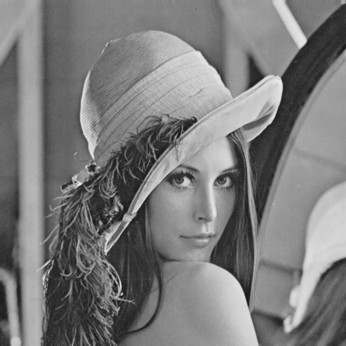
\includegraphics[width=0.45\linewidth]{figs/lena.jpg}(a)
	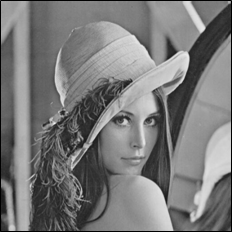
\includegraphics[width=0.45\linewidth]{figs/lenaSigma1.png}(b)
	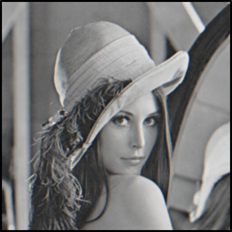
\includegraphics[width=0.45\linewidth]{figs/lenaSigma2.png}(c)
 	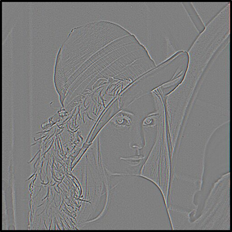
\includegraphics[width=0.45\linewidth]{figs/lenaDoG.png} (d)
	\caption{%
	É aplicado um filtro gaussiano na imagem original (a), com $\sigma$ = 1, tendo como resultado a imagem (b).
	Um outro filtro gaussiano é usado, porém, neste caso, o $\sigma$ = 2 (c). Após isso, subtrai-se (b) de (c), obtendo 
	o filtro DoG (d).
	}\label{fig:lenadog}
\end{figure}

Uma vez que o Dog é aplicado, as iamgens são utilizadas com o espaço e escala extremos. Por exemplo, na imagem \ref{fig:extrema}, um pixel é comparado com seus 8 vizinhos, assim como comparado com os 9 pixels na próxima escala e os 9 pixels na escala anterior. Se esse pixel é um local extremo, ele é um ponto chave em potencial. Isto é, este ponto chave é melhor representado nesta escala.

\begin{figure} [!h]
	\centering
	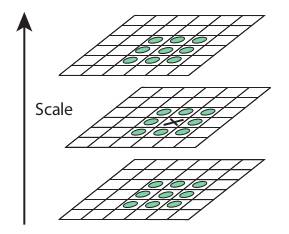
\includegraphics[width=0.45\linewidth]{figs/sift_local_extrema.jpg}
	\caption{%
	Exemplo de funcionamento de deteccão de espaço de escala extrema
	}\label{fig:extrema}
\end{figure}

No caso, as funções ficariam da seguinte forma: 

\begin{equation}
	g_\sigma(x) = \frac{1}{2 \pi \sigma ^2} e^{-\frac{1}{2} \frac{x^T x}{\sigma ^2}}
	\label{eq:gaussiano}
\end{equation}

\begin{equation}
	I_\sigma = g_\sigma * I, \sigma >= 0

\label{eq:gaussianScaleSpace}
\end{equation}

\begin{equation}
\triangledown^2	g_\sigma(x)
	\label{eq:LoG}
\end{equation}

\begin{equation}
	DoG_\sigma(o,s) = I_\sigma(o,s+1) - I_\sigma(o,s)
	\label{eq:DoG}
\end{equation}


Onde \ref{eq:gaussiano} é a função padrão do operador gaussiano (núcleo), a equação \ref{eq:LoG} é o operador LoG,  \ref{eq:DoG} é o operador DoG e $\triangledown^2$ é o operador Laplaciano.

\subsection{Localização de pontos chaves}

A localização dos pontos extremos pode cair em um extremo local e não global. Logo, após a utilização do DoG e com os pontos chaves em potencial localizados, eles precisam ser refinados para melhorar o resultado. Para isso, são utilizadas Séries de Taylor na escala e no espaço, e, se a intensidade nesse extremo é menor que o valor limite, este é rejeitado.
%TODO: Ver isso 
Os {\it frames} do SIFT (pontos chaves) são extraídos baseados nos extremos locais (picos) a partir do DoG. Numericamente, extremos locais são elementos que possuem um menor (ou maior) valor em uma vizinhança em um espaço 3x3x3 (em escala e espaço).
Depois de extraídos, estes pontos são interpolados quadraticamente (este passo é muito importante, especialmente nas escalas de menor resolução, para ter uma localização precisa do ponto chave na resolução completa). Finalmente, eles são filtrados para eliminar respostas de baixo contraste ou respostas próximas as bordas.

%Eliminating low contrast responses

Picos que são pequenos, na maior parte das vezes são gerados a partir de ruídos e necessitam ser descartados também. Isso é feito com uma comparação de valor absoluto do DoG no pico com o valor do pico limite e é descartado caso este valor é menor que o limite.


%Eliminating edge responses

Para eliminar respostas em bordas, normalmente os picos mais rasos ou horizontais, são gerados por bordas e não possuem características estáveis, portanto estes picos precisam ser removidos. Para isso, dado um pico (x,y, $\sigma$), o algoritmo avalia a matriz Hessiana (x,y) do DoG na escala $\sigma$. Então é computado um valor para esta equação (\ref{eq:hessianaDoG}):

\begin{equation}
	v = \frac{( L_p \space D(x,y,\sigma))^2}{Det \space D(x,y,\sigma)}
	\label{eq:hessianaDoG}
\end{equation}

Onde,

D = \begin{bmatrix}
	\frac{\partial ^2 DoG}{\partial x^2} & \frac{\partial ^2 DoG}{\partial x \partial y} \\ 
	\frac{\partial ^2 DoG}{\partial x \partial y} & \frac{\partial ^2 DoG}{\partial y^2} 
\end{bmatrix}
 
No caso, v possui um valor mínimo (igual a 4) quando os autovalores da Jacobiana são iguais (pico curvado) e aumentam à medida que um dos autovalores aumenta e os outros permanecem baixos. Os picos são retidos se $v  < \frac{(t_e+1)(t_e+1)}{t_e}$ , onde $t_e$ é o limite da borda. 

% This score has a minimum (equal to 4) when both eigenvalues of the Jacobian are equal (curved peak) and increases as one of the eigenvalues grows and the other stays small. Peaks are retained if the score is below the quantity (te+1)(te+1)/te(te+1)(te+1)/te, where tete is the edge threshold. Notice that this quantity has a minimum equal to 4 when te=1te=1 and grows thereafter. Therefore the range of the edge threshold is [1,∞)[1,∞).

% Peaks which are too short may have been generated by noise and are discarded. This is done by comparing the absolute value of the DoG scale space at the peak with the peak threshold tptp and discarding the peak its value is below the threshold.


% O DoG tem respostas altas nas bordas, então, precisam ser removidas. Para isso, um conceito similar ao algoritmo de Harris para detecção de bordas é utilizado: uma matriz Hessiana 2x2 (H) é usada para computar a curvatura principal.

% Once potential keypoints locations are found, they have to be refined to get more accurate results. They used Taylor series expansion of scale space to get more accurate location of extrema, and if the intensity at this extrema is less than a threshold value (0.03 as per the paper), it is rejected. This threshold is called contrastThreshold in OpenCV

% DoG has higher response for edges, so edges also need to be removed. For this, a concept similar to Harris corner detector is used. They used a 2x2 Hessian matrix (H) to compute the pricipal curvature. We know from Harris corner detector that for edges, one eigen value is larger than the other. So here they used a simple function,

% If this ratio is greater than a threshold, called edgeThreshold in OpenCV, that keypoint is discarded. It is given as 10 in paper.

% So it eliminates any low-contrast keypoints and edge keypoints and what remains is strong interest points.


%No presente trabalho, nos concentramos na configuração do tanque de onda
%oceânica descrita na Seção~\ref{sec:setup}, composta por quatro vídeos
%\emph{Full HD} tirados de diferentes pontos de vista em widebaseline. Cada vídeo tem cerca de 300 MB de
%resolução 1920x1080 e 30 fps.
%
%\section {Arquitetura de Implementação}
%
%Nosso sistema prático foi projetado para C++ usando as bibliotecas de visão 
%computacional VXL e VXD~\cite{vxl,vxd}. A linguagem C++ é rápida e escalável, e muitas
%vezes é a única solução para as grandes quantidades de processamento de vídeo que
%visamos. Além disto, escolhemos utilizar uma solução baseada em VXL por ser
%amplamenta utilizada na indústria, pela sua suite de testes e, também, por
%prover a opção de utilizar OpenCV caso necessário. A VXL é internamente utilizada
%por empresas como a General Electrics, a Vision Systems Inc, a Google, e uma
%série de startups e universidades, para sistemas de visão maiores e mais
%experimentais do que o OpenCV.
%
%Na prática, no entanto, foram apenas implementados os filtros treinados finais e
%os sinais (\emph{features}) em C++, com base no código Matlab de referência
%por~\etal~\cite{Guo:etal:CVPR14,Guo:etal:PAMI2017:submitted}. Nosso código 
%C++ é aberto na biblioteca VXD e já foi usado pela
%Brown University e outros pacotes~\cite{Yuliang:edge:detection:github}. Decidimos 
%manter o treinamento dos
%classificadores topológicos de fragmentos de curva em Matlab, pois queríamos
%experimentar muito com ele usando a interatividade fornecida por essa linguagem
%``lab''. O código Matlab é baseado no código original de
%Guo~\etal~\cite{Guo:etal:CVPR14,Guo:etal:PAMI2017:submitted}.
%
%O processamento C++ foi implementado em paralelo, usando um nível UNIX
%de granularidade de comunicação. Na implementação atual, cada processo atua em
%dados de um único quadro de vídeo separadamente, em um único nó, usando
%múltiplos núcleos. O paralelismo de nível de processo é programado de forma
%flexível e programável para pesquisa, o GNU
%Parallel~\cite{Tange:GNU:Parallel:USENIX2011}, que também pode usar
%múltiplos nós como no MPI.
%
%Este nível de granularidade foi mais do que suficiente para acelerar nosso
%processamento de vídeo e protótipo do sistema, mas \emph{multithreading} através do
%paradigma de fluxo de dados também é uma possibilidade, pois usamos a
%mesma tecnologia subjacente que o sistema 3D Curve Sketch
%Multithread~\cite{Fabbri:Kimia:CVPR10}.
%
%Além disso, o paralelismo de nível de processo simples é bastante poderoso,
%robusto, programável e extensível, ao longo da tradição UNIX de dividir um
%sistema grande em pequenos programas independentes. É favorável à distribuição
%futura através do MPI e tecnologias relacionadas, enquanto o código interno para
%cada processo é acessível por níveis de granularidades mais finos através do
%CUDA; Os processos podem acelerar a comunicação através da memória ou dos pipes
%compartilhados em vez da abordagem baseada em arquivos atual. O custo da criação
%do processo é insignificante cada vez que os dados são lidos por quadro, uma vez
%que as imagens e o vídeo multivisão são muito ``big data''.
%
%\section {Processamento inicial}
%
%Cada um dos quatro vídeos de 3min é convertido em 182 arquivos de imagem PNG, um
%por quadro, usando o software de processamento de vídeo multithreaded de baixo nível
%FFmpeg~\cite{FFmpegurl}. Isso é adequado para a prototipagem de uma solução de pesquisa, e
%também para uma solução final de processamento em lote (\emph{batch}). Um sistema de produção
%poderia explorar formas de decodificar o vídeo \emph{on-the-fly} usando hardware, se o
%objetivo é o processamento online em tempo real. No entanto, dada a imagem maior
%que nosso rastreador de borda será usado dentro de um sistema de reconstrução 3D
%que usa muitos quadros globalmente no vídeo, extrair quadros em arquivos de
%imagem não é o gargalo.
%
%%\begin{figure}
%%  \centering
%%  \includegraphics[width=\linewidth]{figs/representative-frames.pdf}
%%  \caption{
%%    Video frames representative of the sea state, extracted from the first camera.}
%%  \label{fig:frames}
%%  \ReduceAfterCaptionfigspace
%%\end{figure}
%
%\begin{figure}[ht]
%  \caption{Etapa de pré-processamento de vídeo: regiões de interessse (a, c) e
%    correção de gama automática opcional (d) otimizamos esse problema, mas não
%    é necessário no sistema atual. O sinal de onda está concentrado nos
%    primeiros 40/255 níveis de cinza (16\%) (b). Veja os materiais
%    suplementares para os vídeos.}
%  \centering
%  \includegraphics[width=\linewidth]{figs/roi-gamma.pdf}
%  \source{O autor, 2017.}
%  \label{fig:roigamma}
%  \ReduceAfterCaptionfigspace
%\end{figure}
%
%\section {Processamento de Imagem}
%
%Para permitir o estudo científico dos padrões nos vídeos, recortamos os quadros
%em regiões de interesse (ROIs). As coordenadas desses ROIs atualmente são
%escritas manualmente para processamento paralelo, de modo que as regiões se
%sobrepõem, tanto quanto possível, entre as câmeras.
%
%A informação desejada nos vídeos está concentrada nos primeiros 40 níveis de
%cinza de 255 (16\%), Figura~\ref{fig:roigamma}. Portanto, foram automaticamente 
%recortados e, opcionalmente, realizado
%ajuste automático de gama em cada quadro em paralelo, usando
%ImageMagick~\cite{ImageMagickurl} e
%GNU Parallel~\cite{Tange:GNU:Parallel:USENIX2011}, 
%Figura~\ref{fig:roigamma}. O ImageMagick é conhecido por priorizar a qualidade
%da imagem sobre a velocidade; Na prática, o uso de sua API a partir de C++ não
%resultaria em benefício de desempenho significativo, ao mesmo tempo em que
%diminuiria a robustez do sistema.
%
%Em nossas experiências, observamos que a extração da curva é robusta o
%suficiente para não requerer este passo de ajuste automático de gama. No entanto, incluímos aqui
%para relatar esta descoberta, e também que selecionamos cuidadosamente
%para este conjunto de dados e pode ser um passo útil para outros tipos de
%processamento. É também o melhor filtro automático para fins de visualização
%desses vídeos, entre muitos que avaliamos. O resultado de que a extração da
%curva foi comprovada robusta com um contraste tão fraco em nossos vídeos é um testemunho
%do poder da abordagem do processamento de imagens usando descontinuidades de
%sombreamento, em vez de regiões de luminosidade suave.
%
%\section{Detecção de borda}
%\begin{figure}
%  \caption{Detector de borda de terceira ordem aplicado a um quadro de vídeo.
%    Observe que a informação bruta é puramente localizada nas bordas, com muitos
%    ruídos detectados em artefatos de compressão. O quadro é ajustado em gama
%    (superior), mas nossas experiências mostraram que o detector de borda é
%    robusto o suficiente para funcionar diretamente sem ajuste de gama.}
%  \centering
%  \includegraphics[width=\linewidth]{figs/third-order-sample-zoom.pdf}
%  \source{O autor, 2017.}
%  \label{fig:3o:zoom}
%  \ReduceAfterCaptionfigspace
%\end{figure}
%
%O detector de borda descrito na Seção~\ref{sec:edge:detection} foi codificado em um programa
%independente para ser aplicado em paralelo em cada quadro usando o GNU Parallel.
%Os parâmetros são armazenados em um arquivo XML, e um shell script foi
%escrito para construir e executar o comando GNU Parallel apropriado para
%arquivos PNG de entrada. A saída é um mapa de borda de subpixel no formato EDG, um
%formato de arquivo de texto compactado com gzip com extensão '\texttt{.edg.gz}'.
%
%Conforme mencionado no Capítulo~\ref{sec:cfrag:extraction}, nossa estratégia é
%estabelecer um limiar de
%baixo contraste para que possamos ter dados de borda brutos com alta cobertura,
%mas muitos falsos positivos a serem filtrados por consistência geométrica pelos
%próximos módulos na pipeline de processamento. A Figura~\ref{fig:3o:zoom} mostra uma amostra
%da detecção de borda inicial com ponto de operação de cobertura ideal para
%nossa aplicação. Observamos que neste limite obtemos alto nível de detalhes nas
%ondas, mas também detectamos muitos artefatos de compressão de vídeo para serem
%removidos mais tarde.
%
%Percebe-se como a imagem de entrada possui bordas muito longas
%geometricamente consistentes com baixo contraste, o que é outra razão pela qual
%precisamos definir os limiares de contraste iniciais muito baixos para permitir
%que o algoritmo de agrupamento geométrico faça o trabalho de escolhê-los. Outro
%benefício de confiar na filtragem geométrica em um nível superior é que a
%estratégia funciona para a maioria dos tipos de imagens sem ter que ajustar
%limiares - basta deixá-los baixos. Isso é confirmado por nossos experimentos,
%onde observamos que o filtro de ajuste automático de gama não é necessário ao iniciar o sistema
%com limiares de contraste muito baixos. Após extensas experiências iniciais, foram
%consertados os parâmetros do detector de borda de terceira ordem de acordo com
%as seguintes regras:
%\begin{itemize}
%  \item Um limite de contraste de '20\% 'foi suficiente para a maioria das
%    aplicações
%  \item Um parâmetro de suavização $\sigma = 2px$ foi considerado o mais útil para
%    aplicações de reconstrução em 3D, mas $\sigma = 3px$ apresentou melhores resultados
%    visuais e uma imagem mais limpa. Esse parâmetro afeta a escala das bordas,
%    mas também introduz a imprecisão de localização, a qual a calibração é
%    sensível. A localização poderia potencialmente ser corrigida ao combinar as
%    bordas em $\sigma = 3px$ com as bordas calculadas por uma escala inferior
%    $\sigma = 2px$,
%    de uma forma multi escala, mas, da nossa experiência, os benefícios
%    potenciais parecem baixos.
%\end{itemize}
%A Figura~\ref{fig:3o:zoom} mostra um resultado de detecção de borda de amostra
%para $\sigma = 3px$.
%
%\section{Extração do contorno inferior}
%Realizamos experimentos extensivos para calcular a saída do agrupamento de borda
%simbólico e suas
%variantes~\cite{Tamrakar:Kimia:ICCV07,Guo:etal:CVPR14,Guo:etal:PAMI2017:submitted}, 
%conforme descrito no Capítulo~\ref{sec:cfrag:extraction}, de início sem o uso
%de qualquer aprendizagem de máquina. Um exemplo de
%quadro do melhor resultado que conseguimos é dado na Figura~\ref{fig:sel:best},
%Seção~\ref{sec:main:results} abaixo. Veja os quatro vídeos no material
%suplementar para perceber as curvas acompanhadas.
%Neste nível de extração de fragmentos de curva, nosso objetivo é produzir alta
%precisão, e secundariamente uma cobertura máxima sem sacrificar a precisão. Alta
%precisão é obrigatória para o estágio inicial das aplicações 3D, uma vez que os
%\emph{outliers} podem sobrecarregar o sistema de inicialização (calibração da câmera e
%correspondência multivisão estéreo); cobertura é desejável, mas apenas para
%completar as reconstruções em uma segunda etapa de reconstrução em 3D.
%
%Em nossas experiências, realizamos um estudo de parâmetros sobre os muitos
%parâmetros internos ao código de extração de fragmentos de curva. A conclusão
%foi que apenas o limiar de comprimento (extensão da consistência geométrica) foi
%significativo. Para uso na primeira fase da reconstrução em 3D, empregou-se um
%limiar de comprimento mais agressivo de 160px (ou seja, apenas foram mantidas
%curvas com comprimento maior ou igual a 160px), representadas na
%Figura~\ref{fig:sel:best}.
%Para tentar aumentar a cobertura, tentamos um limite de comprimento de 80px, mas
%houve mais \emph{outliers} que se ligam aos padrões de ruído de
%compressão de fundo. Para os estágios posteriores da reconstrução,
%gostaríamos de conseguir uma maior cobertura. É por isso que exploramos a abordagem
%baseada em aprendizagem supervisionada como descrito na próxima seção. Outra
%situação em que precisamos melhorar esses resultados é quando o padrão de água
%fica mais quebrado, caso em que o sistema precisa ser robusto o suficiente para
%lidar com curvas menores (assim, maior cobertura) com maior precisão.
%
%Os estágios posteriores das aplicações de reconstrução 3D são capazes de
%filtrar contornos falso-positivos, exigindo que sejam consistentes em várias
%imagens e vídeos. Portanto, em princípio, o sistema pode se beneficiar de maior
%cobertura e menor precisão. Isso, no entanto, supera o custo computacional do
%sistema de correspondência multivisão estéreo. Em cenas desafiadoras, como em
%imagens aquáticas, existem muitos padrões repetitivos, de forma que a alta precisão e
%a cobertura possam ser cruciais como entrada.
%
%\section{Extração de contorno baseada em aprendizagem}
%\begin{figure}[h]
%  \caption{Filtros de união e quebra de contorno geométrico: exemplos de efeitos.}
%  \centering
%  \includegraphics[width=\linewidth]{figs/break-merge-zoom.pdf}
%  \source{O autor, 2017.}
%  \label{fig:break:merge:sample}
%  \ReduceAfterCaptionfigspace
%\end{figure}
%
%Os filtros de quebra e união geométricos descritos no
%Capítulo~\ref{sec:cfrag:extraction} foram aplicados
%na tentativa de aumentar o nível de detalhes (cobertura) nos padrões de ondas,
%minimizando falsos positivos (alta precisão). A
%Figura~\ref{fig:break:merge:sample} ilustra os efeitos
%dos filtros de união e quebra em um quadro de imagem real do tanque de ondas de
%água. A Figura~\ref{fig:break:merge:sample} ilustra os efeitos de cada etapa aplicada em seqüência,
%incluindo a união, quebra e remoção baseada em classificação, usando o conjunto de
%treinamento descrito em~\ref{sec:generic:datasets}.
%\begin{figure}
%  \caption{Resultados da amostra de estágios de aprendizagem de máquinas
%  supervisionados.}
%  \centering
%  \includegraphics[width=\linewidth]{figs/learned-results-sample.pdf}\hspace{-1em}
%  \legend{(a) Entrada da geometria do agrupador de borda simbólica
%    crua com alta cobertura; (b) Filtro de quebra aprendido a partir de
%    imagens genéricas naturais (c) Filtro de ranqueamento/classificação aprendido com imagens
%    naturais; (d) Filtro de união aprendido com imagens naturais genéricas.}
%  \source{O autor, 2017.}
%  \label{fig:learned:samples}
%  \ReduceAfterCaptionfigspace
%\end{figure}
%
%
%%\todo{Describe the results using Dayany dataset}
%%\todo{Incluir dados acima na apresentação}
%
%\section{Resultados principais}\label{sec:main:results}
%
%Nossos melhores resultados sem aprendizado são mostrados
%num instante de tempo na Figura~\ref{fig:sel:best}. Estes já são suficientes para entrar em um
%pipeline de reconstucção
%3D~\cite{Fabbri:Kimia:CVPR10,Usumezbas:Fabbri:Kimia:ECCV16,Usumezbas:Fabbri:Kimia:CVPR17}. 
%Consulte os vídeos no material suplementar para analisar todos os
%quadros. Ao aplicar toda a pipeline de processamento aos quatro vídeos de
%entrada, conseguimos melhorar a cobertura sem perda relativa de precisão,
%Figura~\ref{fig:learned:final}.
%
%%/todo{incluir esse dados na apresentação}
%
%\begin{figure}
%  \caption{Os melhores resultados de curva agrupada não supervisionados para
%    reconstrução em 3D e fotogrametria. Os resultados exibem uma alta precisão,
%    mas a cobertura pode ser melhorada (dados faltantes). Veja os vídeos nos
%    materiais suplementares.}
%  \centering
%  \includegraphics[width=\linewidth]{figs/raw-sel-best-result.png}
%  \source{O autor, 2017.}
%  \label{fig:sel:best}
%  \ReduceAfterCaptionfigspace
%\end{figure}
%
%\begin{figure}
%  \caption{Resultados finais de alta cobertura em um quadro de um dos quatro
%    vídeos. Veja o material suplementar para os vídeos.}
%  \centering
%  \includegraphics[width=\linewidth]{figs/final-high-recall-results.pdf}
%  \source{O autor, 2017.}
%  \label{fig:learned:final}
%  \ReduceAfterCaptionfigspace
%\end{figure}

\chapter{Experimentos}\label{sec:experiments}
%======================================================================================
No presente trabalho, nos concentramos no objetivo proposto descrito na Seção~\ref{sec:objetivos}.

\section{Procedimento}
Primeiramente, filmamos algumas esculturas utilizando a câmera de um \emph{smartphone} convencional na resolução de 1920x1080 pixels. Esta filmagem foi realizada varrendo toda (ou maioria) da superfície da escultura em $360^{\circ}$ com o intuito de ter toda a escultura reconstruída \ref{fig:procedimentoscan}.
Após isso, fizemos mais alguns vídeos, pegando alguns pontos que possuíam mais detalhes e que, com uma única varredura, não era capaz de reproduzir uma boa reconstrução.

\begin{figure}[!h]
	\centering
	%   \includegraphics[width=1.0\linewidth]{figs/3d-curve-sketch/system-diagram.eps}
	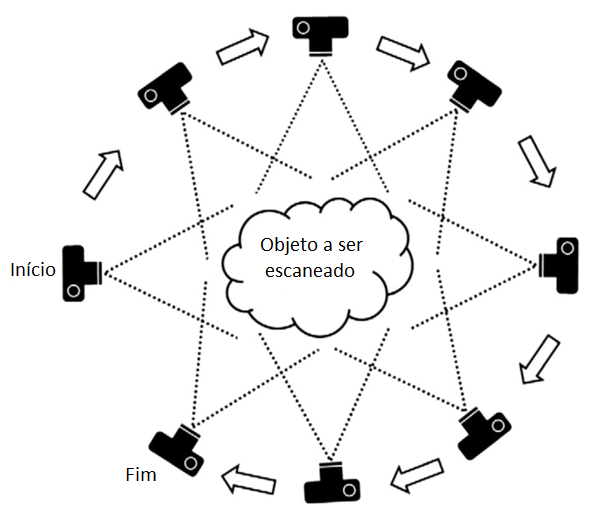
\includegraphics[width=0.4\linewidth]{figs/procedimentoscan.png}
	\caption{%
	Exemplo de como foi realizada a varredura da escultura
	%\cite{Cui:Theobalt:etal:PAMI2013,Pajdla:etal:ICCV2011}.
	}\label{fig:procedimentoscan}
\end{figure}

Com este material, foram feitos "cortes" em determinados \emph{frames} do vídeo, com atenção para não cortar em \emph{frames} muito juntos, pois aumentaria o número de correspondências ambíguas entre as imagens e com isso, o processamento da reconstrução demoraria mais. E não usar \emph{frames} muito distantes, que ocorreria o inverso: com menos correspondências, ficariam buracos (partes sem a informação necessária) na reconstrução, como descrito na Seção \ref{sec:mve}.

Com isso em mente, foram reconstruídas duas esculturas: empregando o VisualSfM, usamos um único vídeo, totalizando 197 imagens. %guerreiro, indio%
Com o MVE, utilizamos dois vídeos, que, ao cortá-los, totalizou cerca de 280 imagens. %sapo%

Além de esculturas ao ar livre, fizemos alguns testes em ambiente fechado, dentro de uma casa, por exemplo. Foi utilizado um objeto feito de cabaça (casca de abóbora) na qual possui uma superfície propícia (Lambertiana)~\cite{basri2003lambertian} para uma reconstrução.

Com o procedimento descrito anteriormente, a partir dos vídeos feitos, obtemos um total de 200 imagens em um vídeo superficial e mais 24 imagens mais detalhadas do objeto, ambos numa resolução de 1080x1920 pixels. E, para um mesmo conjunto de imagens, rodamos tanto o VisualSfM quanto o MVE.

\subsection{Resultados da reconstrução com o VisualSfM}

Seguindo o passo-a-passo de reconstrução do software, obtivemos os seguintes resultados, para a escultura de 197 imagens do Jardim do Nêgo.

\begin{table}[h!]
\caption{Tempos obtidos da reconstrução da escultura do Jardim do Nêgo usando o VisualSfM}
\label{tab:temposSfMJardimDoNego}
\begin{tabular}{|l|p{4.7cm}|}
\hline
Procedimento & Tempo (aprox.) \\ \hline
Carregamento de imagens & 10 segundos \\ \hline
Calcular pares correspondentes de \emph{features} & 6.643 segundos \\ \hline
Gerar a reconstrução esparsa do modelo & 220 segundos \\ \hline
Gerar a reconstrução densa do modelo & 1.385 segundos \\ \hline
\end{tabular}
\end{table}

Com as seguintes reconstruções~\ref{fig:reconstrucaoEsparsaIndioVisualSFM},~\ref{fig:reconstrucaoDensaIndioVisualSFM}.
Percebemos que foi gerada uma nuvem de pontos bem consistente, a partir da reconstrução esparsa do algoritmo PBA.
Por conta disso, nossa reconstrução 3D densa, empregando o MCBA/PMVS-2 obteve uma qualidade adequada para o conjunto de imagens usada.
%COLOCAR IMAGENS GUERREIRO AQUI%

\begin{figure}[!h]
	\centering
	%   \includegraphics[width=1.0\linewidth]{figs/3d-curve-sketch/system-diagram.eps}
	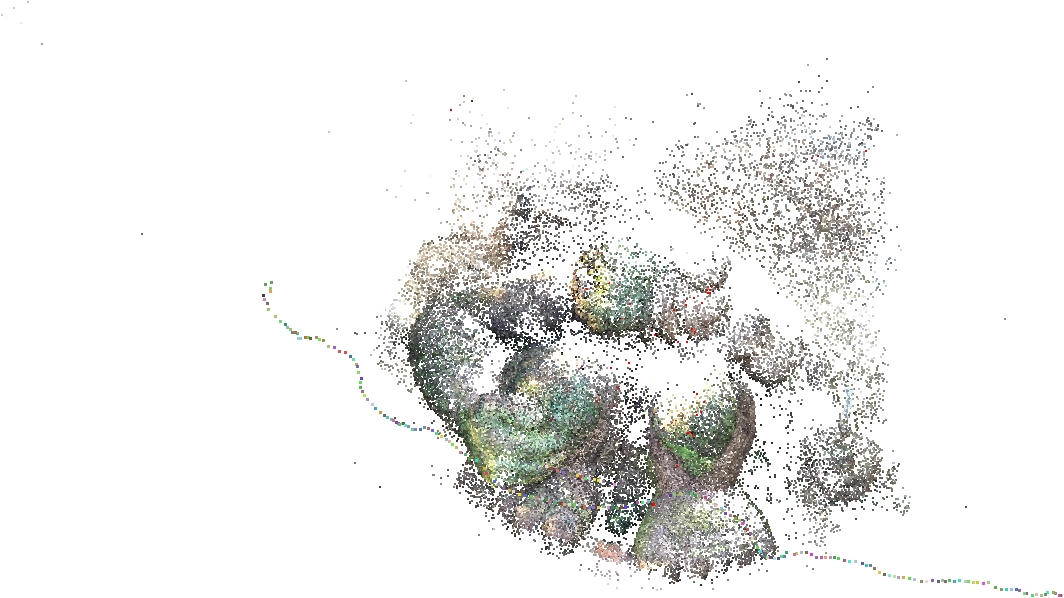
\includegraphics[width=0.9\linewidth]{figs/guerreiroEsparsa.jpg}
	\caption{%
	Reconstrução esparsa da escultura do Jardim do Nêgo no VisualSfM com 197 imagens.
	%\cite{Cui:Theobalt:etal:PAMI2013,Pajdla:etal:ICCV2011}.
	}\label{fig:reconstrucaoEsparsaIndioVisualSFM}
\end{figure}

\newpage

\begin{figure}[!h]
	\centering
	%   \includegraphics[width=1.0\linewidth]{figs/3d-curve-sketch/system-diagram.eps}
	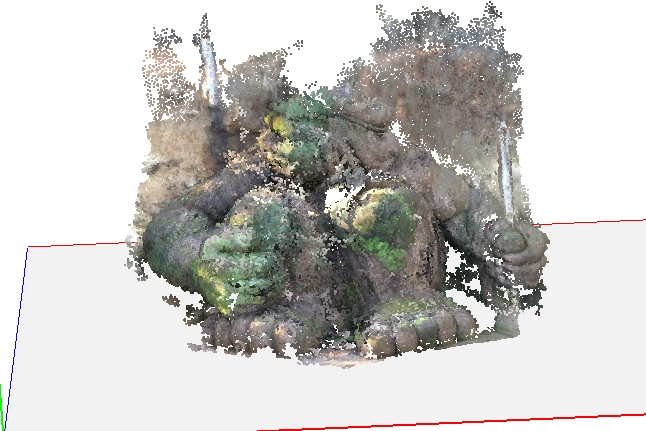
\includegraphics[width=0.40\linewidth]{figs/guerreirovisualsfmdmr.jpg}(a)
	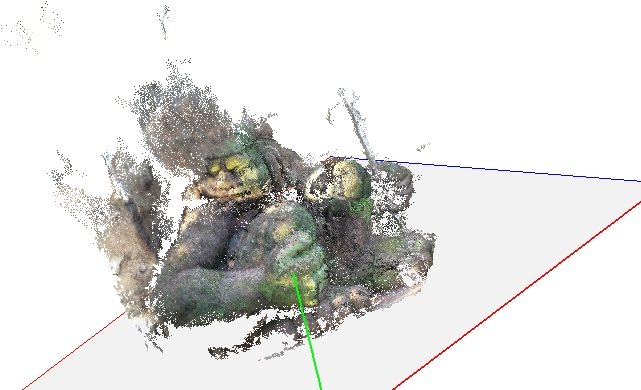
\includegraphics[width=0.50\linewidth]{figs/guerreirovisualsfmdmr2.jpg}(b)
	\caption{%
	Resultados da reconstrução densa da escultura do Jardim do Nêgo usando o VisualSfM, em dois ângulos diferentes (a) e (b).
	%\cite{Cui:Theobalt:etal:PAMI2013,Pajdla:etal:ICCV2011}.
	}\label{fig:reconstrucaoDensaIndioVisualSFM}
\end{figure}


%-------------------GALINHA A PARTIR DAQUI----------------------------------%

Com o objeto em ambiente fechado, conseguimos os resultados a seguir. 

Para o primeiro vídeo, convertido em 200 imagens:

\begin{table}[h!]
\caption{Tempos obtidos da reconstrução do objeto, com 200 imagens usando o VisualSfM}
\label{tab:temposSfM}
\begin{tabular}{|l|p{4.7cm}|}
\hline
Procedimento & Tempo (aprox.) \\ \hline
Carregamento de imagens & 50 segundos \\ \hline
Calcular pares correspondentes de \emph{features} & 9.540 segundos \\ \hline
Gerar a reconstrução esparsa do modelo & 135 segundos \\ \hline
Gerar a reconstrução densa do modelo & 1.416 segundos \\ \hline
\end{tabular}
\end{table}

A Figura~\ref{fig:reconstrucaoEsparsaVisualSFM} mostra o resultado da
reconstrução esparsa do algoritmo PBA. Não é tão nítida como na reconstrução
densa, Figura~\ref{fig:reconstrucaoDensaVisualSFM}, a quantidade de ruídos,
provenientes de outros objetos presentes na cena (o VisualSfM só identifica
objetos estáticos). Só é possível limpar a malha manualmente, pressionando a
tecla F1 e selecionando a área desejada para ser deletada. Não é muito prático,
pois podemos excluir alguns pontos importantes, o ideal seria fazer esta limpeza
por meio de programas externos.

\begin{figure}[!h]
	\centering
	%   \includegraphics[width=1.0\linewidth]{figs/3d-curve-sketch/system-diagram.eps}
	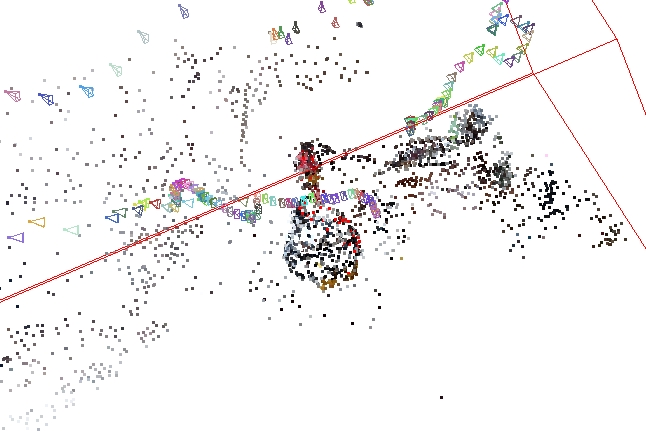
\includegraphics[width=0.5\linewidth]{figs/galinhasparsa.jpg}
	\caption{%
	Reconstrução esparsa do objeto no VisualSfM com 200 imagens.
	%\cite{Cui:Theobalt:etal:PAMI2013,Pajdla:etal:ICCV2011}.
	}\label{fig:reconstrucaoEsparsaVisualSFM}
\end{figure}

\begin{figure}[!h]
	\centering
	%   \includegraphics[width=1.0\linewidth]{figs/3d-curve-sketch/system-diagram.eps}
	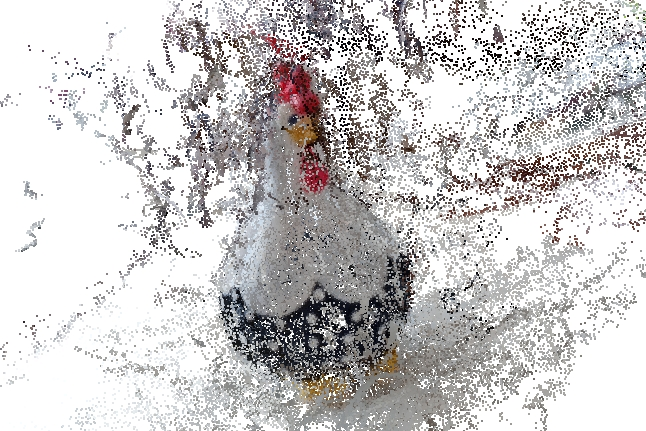
\includegraphics[width=\linewidth]{figs/galinhadense.jpg}
	\caption{%
	Reconstrução densa do objeto no VisualSfM com 200 imagens.
	%\cite{Cui:Theobalt:etal:PAMI2013,Pajdla:etal:ICCV2011}.
	}\label{fig:reconstrucaoDensaVisualSFM}
\end{figure}

Fizemos uma outra reconstrução, utilizando os dois vídeos (gerando 224 imagens). Caso usássemos um conjunto maior, o programa parava de funcionar por falta de memória, mesmo após ajustar parâmetros (como o número de vizinhos, número de \emph{cores} do processador, \emph{level} do PMVS, entre outros) para melhorar esse problema. Portanto, o experimento seguiu da forma:

\begin{table}[h!]
\caption{Tempos obtidos da reconstrução do objeto, com 224 imagens usando o VisualSfM}
\label{tab:temposSfM224}
\begin{tabular}{|l|p{4.7cm}|}
\hline
Procedimento & Tempo (aprox.) \\ \hline
Carregamento de imagens & 60 segundos \\ \hline
Calcular pares correspondentes de \emph{features} & 10.451 segundos \\ \hline
Gerar a reconstrução esparsa do modelo & 162 segundos \\ \hline
Gerar a reconstrução densa do modelo & 1920 segundos \\ \hline
\end{tabular}
\end{table}

Percebemos que não foi tão proveitoso (qualitativamente) usar mais imagens neste
caso, inclusive o algoritmo perdeu a referência do objeto e gerou um segundo
modelo na reconstrução esparsa,
Figura~\ref{fig:reconstrucaoEsparsaVisualSFM224}, e, consequentemente, na
reconstrução densa,
Figuras~\ref{fig:reconstrucaoDensaVisualSFM2241},~\ref{fig:reconstrucaoDensaVisualSFM2241:2} e~\ref{fig:reconstrucaoDensaVisualSFM2242}. O que gerou uma certa incoerência na reconstrução.

\begin{figure}[!h]
	\centering
	%   \includegraphics[width=1.0\linewidth]{figs/3d-curve-sketch/system-diagram.eps}
	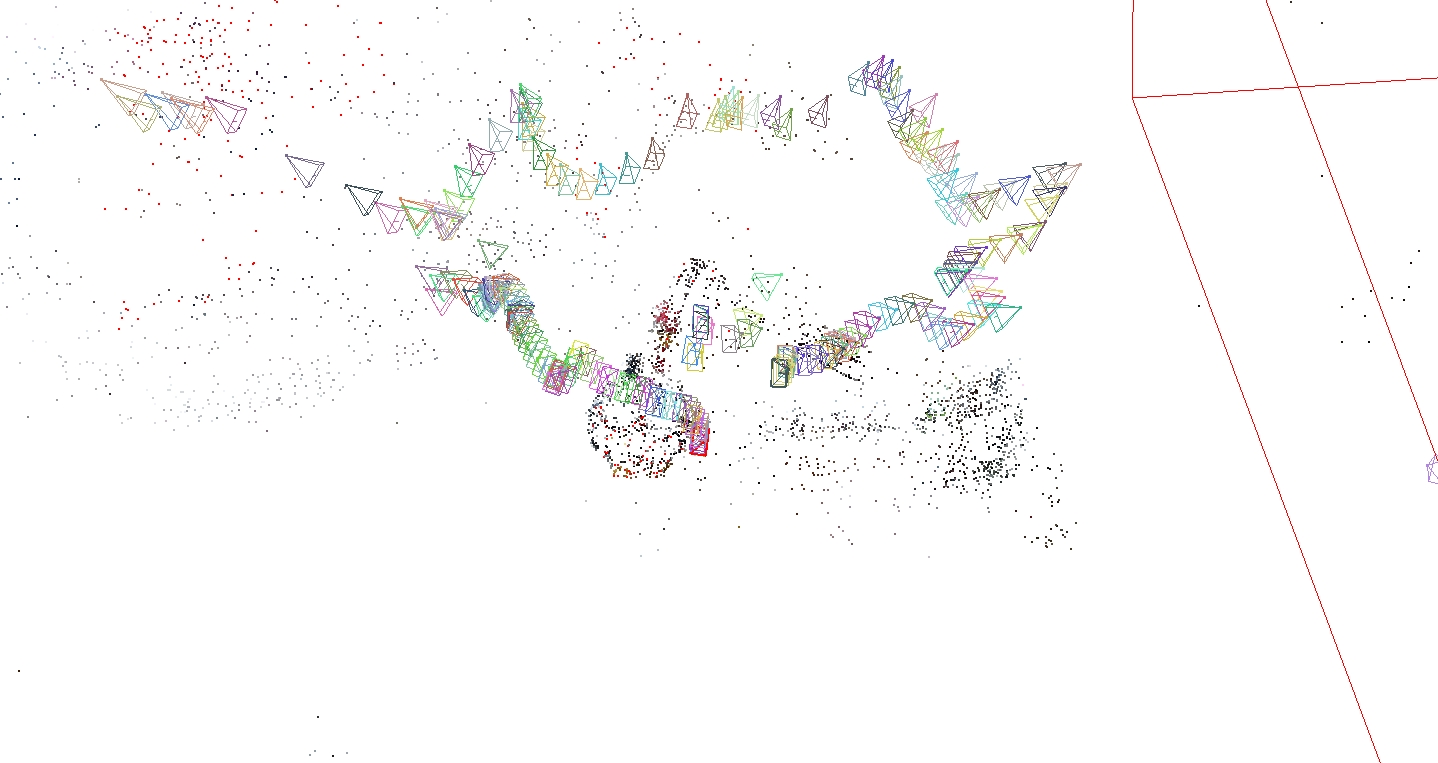
\includegraphics[width=\linewidth]{figs/perto_longe_esparsa.jpg}
	\caption{%
	Reconstrução esparsa do objeto com 224 imagens no VisualSfM.
	%\cite{Cui:Theobalt:etal:PAMI2013,Pajdla:etal:ICCV2011}.
	}\label{fig:reconstrucaoEsparsaVisualSFM224}
\end{figure}

\begin{figure}[!h]
	\centering
	%   \includegraphics[width=1.0\linewidth]{figs/3d-curve-sketch/system-diagram.eps}
	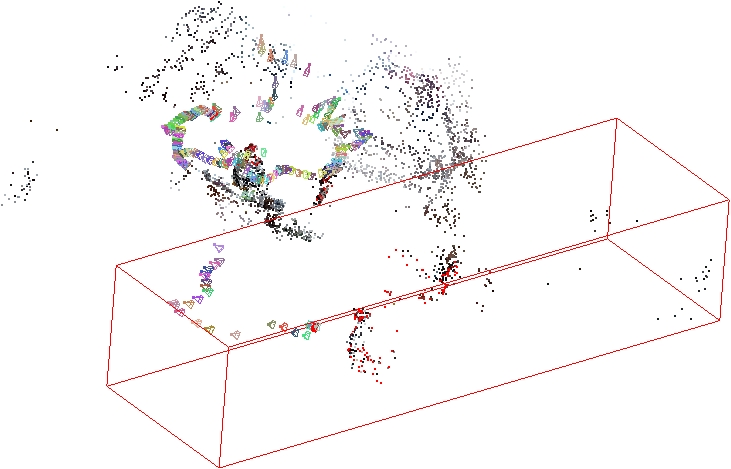
\includegraphics[width=\linewidth]{figs/perto_longe_esparsa_2.jpg}
	\caption{%
	Caso em que foram gerados dois modelos refletidos esparsos do objeto a partir
  do conjunto inicial de 224 imagens, provavelmente, proveniente da falta de
  informações para estimar as câmeras.
	%\cite{Cui:Theobalt:etal:PAMI2013,Pajdla:etal:ICCV2011}.
	}\label{fig:reconstrucaoEsparsaVisualSFM224:2}
\end{figure}

\begin{figure}[!h]
	\centering
	\subfloat[]{\label{fig:reconstrucaoDensaVisualSFM2241}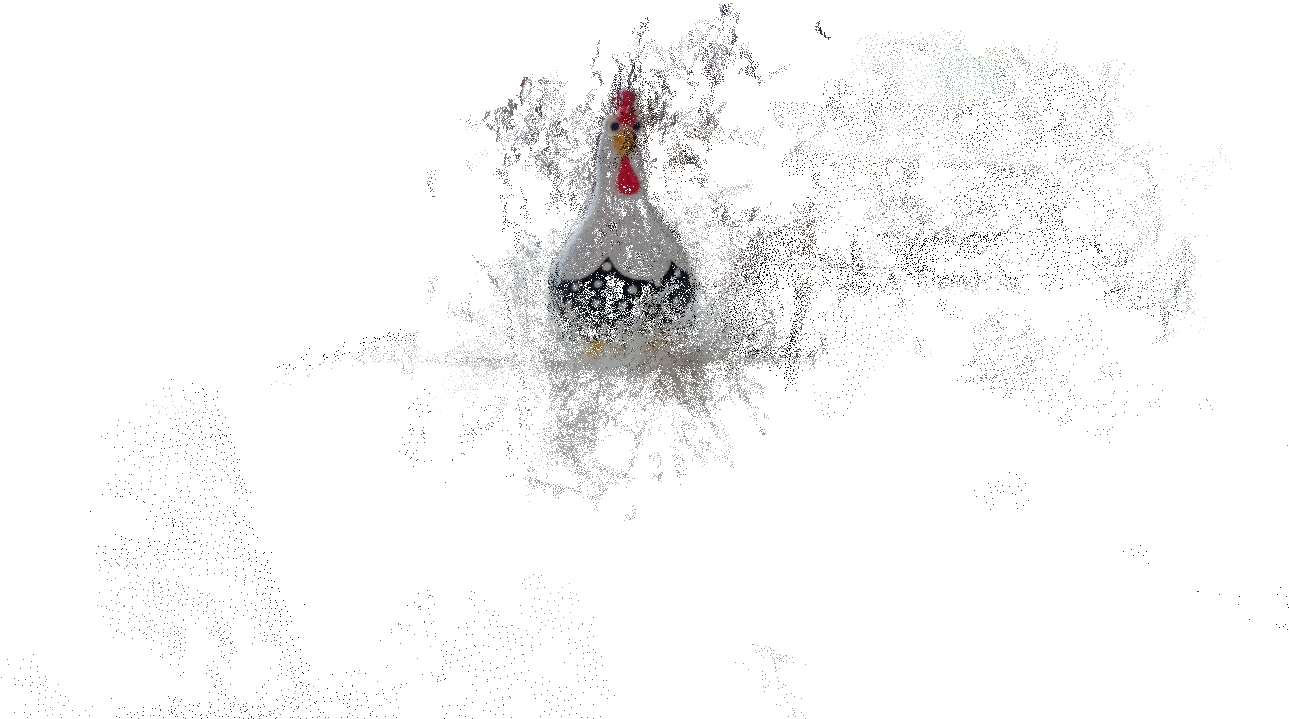
\includegraphics[width=0.5\linewidth]{figs/galinhadense224.jpg}}
	\subfloat[]{\label{fig:reconstrucaoDensaVisualSFM2242}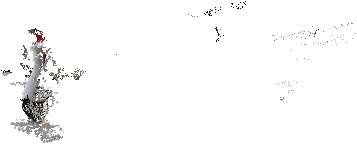
\includegraphics[width=0.5\linewidth]{figs/galinhavisualsfm224.jpg}}
	\caption{Reconstruções densas do primeiro (a) e do segundo (b) modelo do objeto no VisualSfM com 224 imagens.
	}
\end{figure}

%------------------ACABOU SFM---------------------------------------------%

\subsection{Resultados da reconstrução com o MVE}

A utilização do software é bem intuitiva, seja por linha de comando ou pela interface gráfica (neste modo, fica mais fácil visualizar cada etapa da reconstrução). Amplamente configurável, podendo escolher a vizinhança, escala, manter o mapa de profundidade, ver os dados \emph{EXIF} de cada imagem, dentre outras configurações.

Entretanto, para a aplicação proposta neste projeto, não é muito interessante, visto que ele utiliza a informação das câmeras, inseridas nas imagens (\emph{EXIF}) e como as imagens empregadas na reconstrução são, tecnicamente, vídeos cortados em determinados \emph{frames}, não é possível obter a informação das câmeras~\ref{fig:mveexif}. Logo o software não tem tanta aplicabilidade neste caso, pois pode recair no problema dos parâmetros padrões adotados para as câmeras não serem bons o suficiente para estes conjuntos de dados. A menos que sejam tiradas fotos sequenciais de alguma escultura ou objeto que se deseja gerar a reconstrução densa, pois dessa forma, as informações necessárias das câmeras estarão armazenadas.

\begin{figure}[!h]
	\centering
	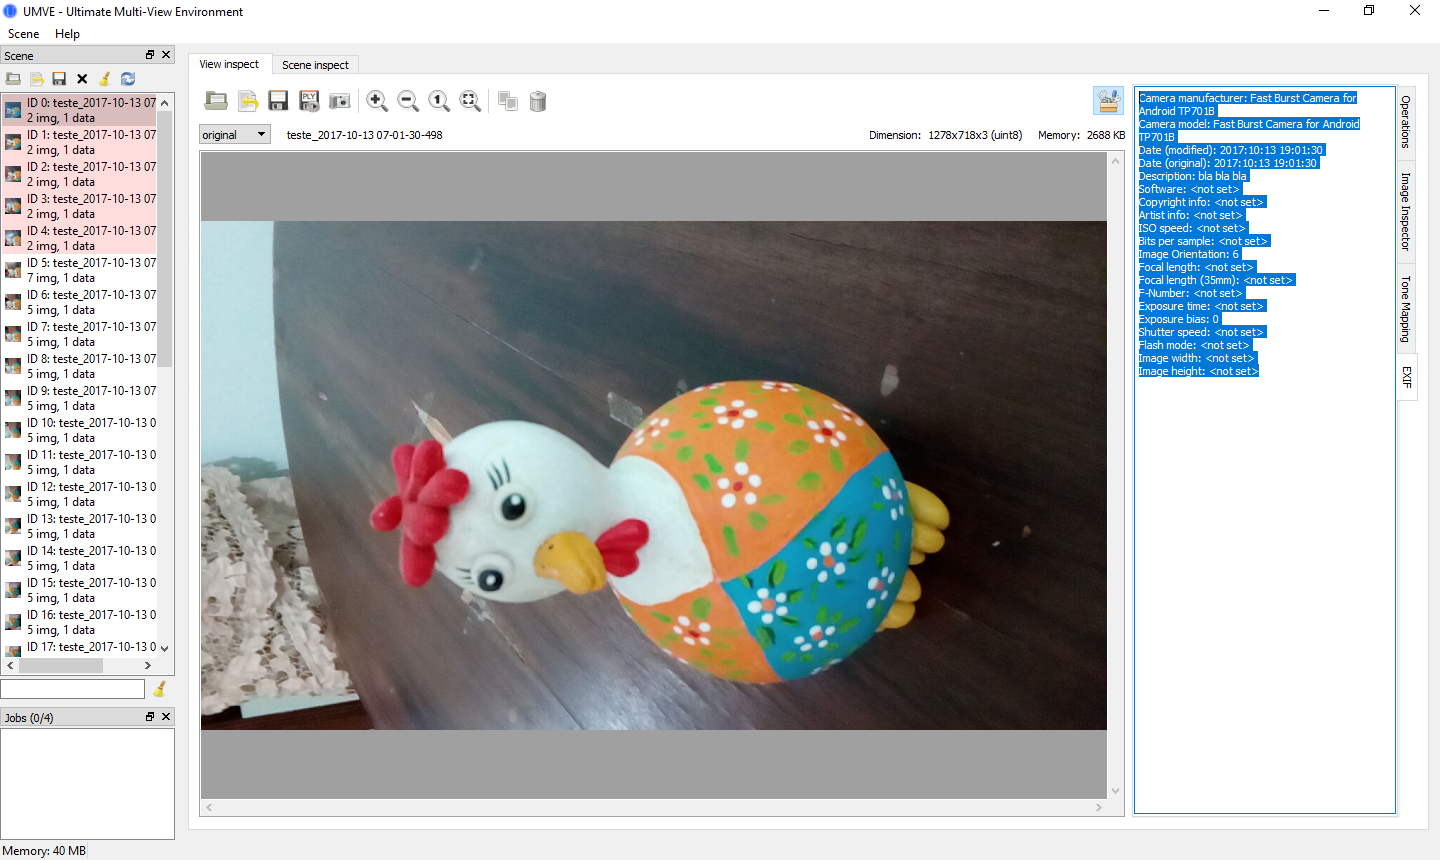
\includegraphics[width=0.461\linewidth]{figs/exifumve.png}(a)
	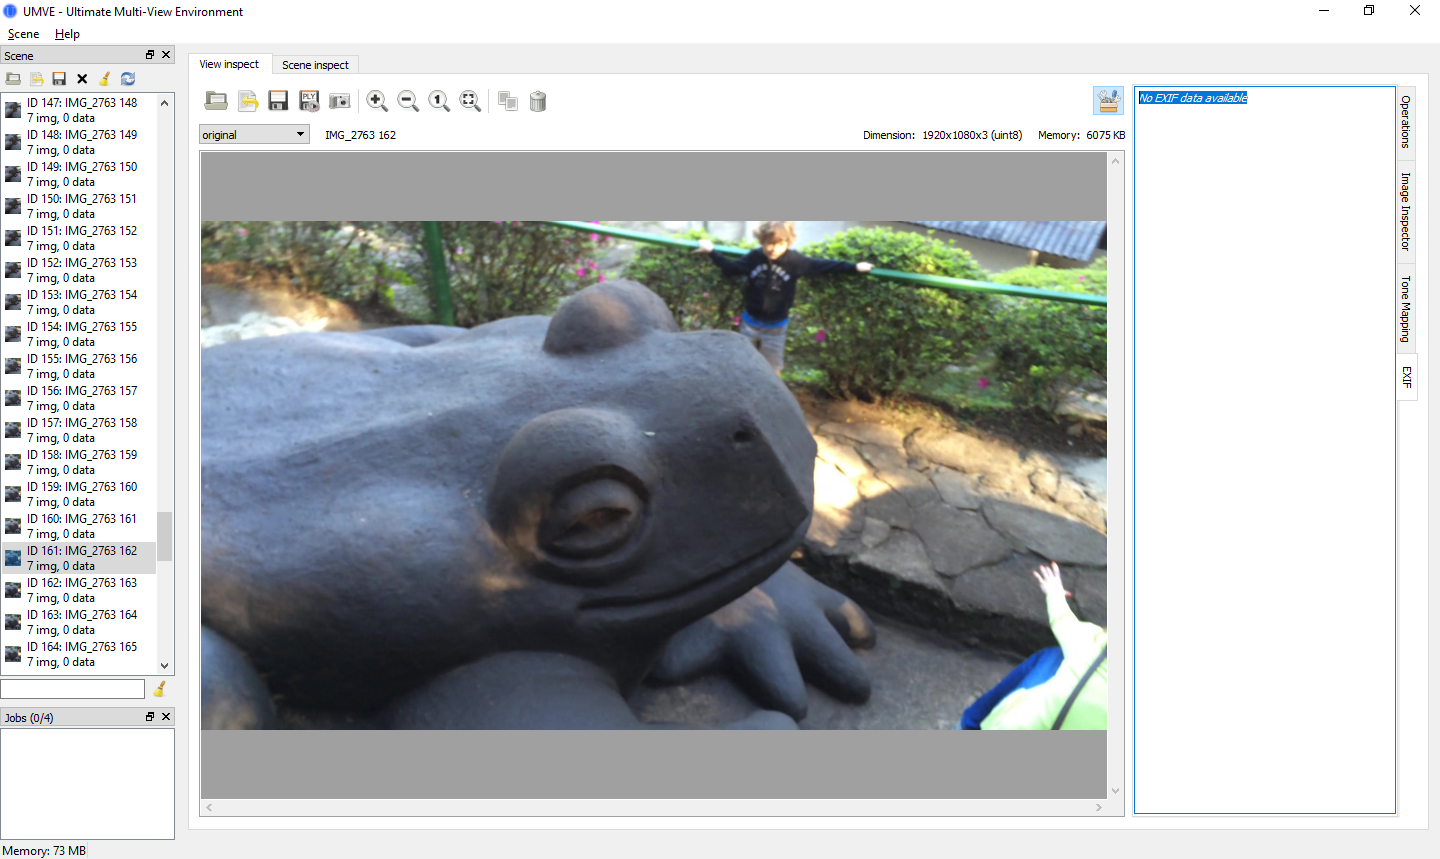
\includegraphics[width=0.461\linewidth]{figs/exifsemumve.png}(b)
	\caption{%
	A figura (a) é um exemplo onde a imagem possui dados na extensão \emph{EXIF} (destacado em azul). Ao passo que a figura (b) é um frame de um vídeo, que não possui os dados das câmeras (destacado em azul).
	%\cite{Cui:Theobalt:etal:PAMI2013,Pajdla:etal:ICCV2011}.
	}\label{fig:mveexif}
\end{figure} 

\newpage

Foi gerada uma reconstrução de um vídeo gravado de uma escultura no Jardim do Nêgo. O  vídeo foi cortado em \emph{frames} onde foram geradas 200 imagens base, com os parâmetros de câmera gerados pelo próprio software. 

A partir disso, foi executado, todos os passos de uma reconstrução utilizando o MVE, de forma que, foram utilizadas as duas opções, tanto por linha de comando, quanto pela interface gráfica (UMVE).

Pela interface gráfica, o processo todo de reconstrução foi rápido (cerca de 30 minutos) \ref{fig:UMVEdense}, ao passo que por linha de comando, levou cerca de 11 horas e 30 minutos, portanto, vamos nos atentar somente à reconstrução por linha de comando, onde, resumindo, tivemos os resultados~\ref{tab:mveSapo}. 

O UMVE não sinaliza quando o processo em execução termina, então, a explicação para essa discrepância no tempo é devido à execução de outro comando, sobrepondo o que já estava sendo executado, sem que o primeiro tivesse terminado.

\begin{figure}[!h]
	\centering
	\includegraphics[width=\linewidth]{figs/umvedense.png}
	\caption{%
  Reconstrução final via UMVE; percebe-se que alguns pontos não foram
  considerados, mas o resultado geral foi uma nuvem de pontos mais densa.
  %\cite{Cui:Theobalt:etal:PAMI2013,Pajdla:etal:ICCV2011}.
	}\label{fig:UMVEdense}
\end{figure} 

\begin{table}[!h]
\centering
\caption{Tempos obtidos usando o MVE em um conjunto de dados do Jardim do Nêgo}
\label{tab:mveSapo}
\begin{tabular}{|l|l|}
\hline
Comando            & Tempo (aprox.)    \\ \hline
\emph{sfmrecon}  & 78 segundos     \\ \hline
\emph{dmrecon}   & 14.503 segundos \\ \hline
\emph{scene2pset} & 600 segundos    \\ \hline
\emph{fssrecon}  & 25.293 segundos \\ \hline
\emph{meshclean} & 60 segundos     \\ \hline
\end{tabular}
\end{table}

Na reconstrução por linha de comando também é possível visualizar em qual etapa da execução o algoritmo está (figura~\ref{fig:passosMVE}), configurar alguns parâmetros e inclusive mostrar a porcentagem de progresso do comando em execução. Foram executados os comandos declarados nesta seção.  O \emph{sfmrecon} demorou cerca de 1 minuto e meio \ref{fig:MVESfM}. 

\newpage

\begin{figure}[!h]
	\centering
	\includegraphics[width=0.45\linewidth]{figs/umve2sfm.png} (a)
	\includegraphics[width=0.45\linewidth]{figs/umve3sfmfeature.png} (b)
	\includegraphics[width=0.45\linewidth]{figs/umve4ba.png} (c)
	\caption{%
	Processos dentro do comando \emph{sfmrecon}, onde (a) estão sendo detectadas as \emph{features} do conjunto de imagens. Em (b) está computado o \emph{pairwise matching} e em (c) está no processo de \emph{Bundle Adjustment}~\cite{bundleAdjustmentSlide}, usando condições-padrão para as câmeras.
	%\cite{Cui:Theobalt:etal:PAMI2013,Pajdla:etal:ICCV2011}.
	}\label{fig:passosMVE}
\end{figure} 

\begin{figure}[h!]
	\centering
	\includegraphics[width=0.65\linewidth]{figs/sfmmve.png}
	\caption{%
	Término do comando \emph{sfmrecon}, onde demorou cerca de 1 minuto e meio (75509 milisegundos).
	%\cite{Cui:Theobalt:etal:PAMI2013,Pajdla:etal:ICCV2011}.
	}\label{fig:MVESfM}
\end{figure}

O próximo comando, \emph{dmrecon} demorou cerca de 4 horas, usando como configuração um nível L2, com 20 vizinhos \ref{fig:MVEDenseRecon}. 
Usando um nível L0, o algoritmo rodou durante 6 horas aproximadamente e foi cancelado devido à demora na execução. 

\newpage

\begin{figure}[!h]
	\centering
	\includegraphics[width=0.8\linewidth]{figs/umvetempo.png}
	\caption{%
	Término do comando \emph{dmrecon}, onde demorou cerca de 4 horas (14502576 milisegundos).
	%\cite{Cui:Theobalt:etal:PAMI2013,Pajdla:etal:ICCV2011}.
	}\label{fig:MVEDenseRecon}
\end{figure} 

Usando o \emph{scene2pset}, é necessário especificarmos em qual nível estamos reconstruindo e também uma saída válida. Por exemplo: "scene2pset.exe -Fnivel cena output". Onde o nível poderá ser um 0 (-F0), 1 (-F1) e assim por diante, a cena é o \emph{input} e o \emph{output} é um arquivo de extensão configurável, neste caso \emph{.ply} \ref{fig:MVEscene2pset}. Este comando foi rápido, demorou cerca de 10 minutos, levando em conta todos os níveis.

\begin{figure}[!h]
	\centering
	\includegraphics[width=0.8\linewidth]{figs/mvemesh.png}
	\caption{%
	Execução dos comandos \emph{scene2pset}, nos níveis -F0, -F1, -F2 e -F3.
	%\cite{Cui:Theobalt:etal:PAMI2013,Pajdla:etal:ICCV2011}.
	}\label{fig:MVEscene2pset}
\end{figure} 

Para juntar todos os níveis do \emph{scene2pset}, foi usado o \emph{fssrecon}, que gera uma única reconstrução. Este processo demorou bastante, cerca de 7 horas \ref{fig:MVEFSSR}. Que teve como resultado a malha \ref{fig:MVEFSSRMesh}.

\newpage

\begin{figure}[!h]
	\centering
	\includegraphics[width=0.8\linewidth]{figs/mvemeshtempo2.png}
	\caption{%
	Progressão do comando \emph{fssrecon}, onde possui o ETA -- \emph{Estimated Time of Arrival}.
	%\cite{Cui:Theobalt:etal:PAMI2013,Pajdla:etal:ICCV2011}.
	}\label{fig:MVEFSSR}
\end{figure} 

\begin{figure}[!h]
	\centering
	\includegraphics[width=1\linewidth]{figs/mvemeshout.png}
	\caption{%
	Malha com ruídos proveniente do comando \emph{fssrecon}.
	%\cite{Cui:Theobalt:etal:PAMI2013,Pajdla:etal:ICCV2011}.
	}\label{fig:MVEFSSRMesh}
\end{figure} 

Finalmente, basta limpar a malha atual com o comando \emph{meshclean}, onde foi obtido o resultado~\ref{fig:MVEMeshClean}.

\newpage

\begin{figure}[!h]
	\centering
	\includegraphics[width=1\linewidth]{figs/mvemeshclean.png}
	\caption{%
	Resultado final, após a remoção dos ruídos da malha.
	%\cite{Cui:Theobalt:etal:PAMI2013,Pajdla:etal:ICCV2011}.
	}\label{fig:MVEMeshClean}
\end{figure} 

Para comparação, usamos o mesmo objeto utilizado na reconstrução do VisualSfM (a galinha) e fizemos o passo a passo com o MVE: com a interface gráfica (UMVE), criamos uma nova cena e inserimos, primeiramente, as 200 fotos do objeto. Em seguida, utilizando as linhas de comando do MVE, fizemos o procedimento padrão de reconstrução do software. E, obtivemos os seguintes resultados~\ref{tab:galinha200mve}:

\begin{table}[!h]
\centering
\caption{Tempos obtidos usando o MVE em um conjunto de dados em ambiente interno com 200 imagens}
\label{tab:galinha200mve}
\begin{tabular}{|l|l|}
\hline
Comando            & Tempo (aprox.)         \\ \hline
\emph{sfmrecon}  & 371 segundos   \\ \hline
\emph{dmrecon}   & 3.716 segundos \\ \hline
\emph{scene2pset} & 300 segundos   \\ \hline
\emph{fssrecon}  & 1.695 segundos \\ \hline
\emph{meshclean} & 45 segundos    \\ \hline
\end{tabular}
\end{table}

\newpage

\begin{figure}[!h]
	\centering
	\includegraphics[width=0.5\linewidth]{figs/galinhalongesfmreconmve.png}
	\caption{%
	Tempo gasto da etapa \emph{sfmrecon} do MVE
	}\label{fig:sfmrecon1}
\end{figure}

\begin{figure}[!h]
	\centering
	\includegraphics[width=0.5\linewidth]{figs/galinhadmreconmve.png}
	\caption{%
	Tempo da etapa \emph{dmrecon} do MVE
	%\cite{Cui:Theobalt:etal:PAMI2013,Pajdla:etal:ICCV2011}.
	}\label{fig:dmrecon1}
\end{figure}

\begin{figure}[!h]
	\centering
	\includegraphics[width=0.7\linewidth]{figs/mvefssrecongalinha.png}
	\caption{%
	Tempo da etapa \emph{fssrecon} do MVE
	%\cite{Cui:Theobalt:etal:PAMI2013,Pajdla:etal:ICCV2011}.
	}\label{fig:fssrecon}
\end{figure}

\begin{figure}[!h]
	\centering
	\includegraphics[width=0.7\linewidth]{figs/galinhadmr.png}
	\caption{%
	Resultado da etapa \emph{fssrecon} do MVE
	%\cite{Cui:Theobalt:etal:PAMI2013,Pajdla:etal:ICCV2011}.
	}\label{fig:galinhaFssr}
\end{figure}

\begin{figure}[!h]
	\centering
	\includegraphics[width=0.7\linewidth]{figs/galinhameshclean.png}
	\caption{%
	Resultado da etapa \emph{meshclean}, da etapa anterior \ref{fig:galinhaFssr}
	%\cite{Cui:Theobalt:etal:PAMI2013,Pajdla:etal:ICCV2011}.
	}\label{fig:galinhaMeshClean}
\end{figure}

\newpage

A etapa de \emph{scene2pset} demorou cerca de 20 segundos (total). Porém percebemos que a reconstrução não foi satisfatória, o \emph{software} se confundiu, e não conseguiu obter os parâmetros corretos das câmeras utilizadas. A partir disso, o erro se propagou e gerou essa reconstrução acima \ref{fig:galinhaFssr} e \ref{fig:galinhaMeshClean}.

Rodamos também, com as 224 fotos, só foi possível executar o passo \emph{sfmrecon} \ref{fig:galinhaSfM224}, pois o MVE não conseguiu rodar o comando \emph{dmrecon} por algum motivo, e não gerou nenhum resultado para a continuação do algoritmo \ref{fig:galinhaDMR224}.

\begin{figure}[!h]
	\centering
	\includegraphics[width=0.5\linewidth]{figs/mvesfmrecongalinhapertolonge.png}
	\caption{%
	Resultado da etapa \emph{sfmrecon}, com todas as imagens
	%\cite{Cui:Theobalt:etal:PAMI2013,Pajdla:etal:ICCV2011}.
	}\label{fig:galinhaSfM224}
\end{figure}

\begin{figure}[!h]
	\centering
	\includegraphics[width=0.5\linewidth]{figs/mvedmrecongalinhapertolonge.png}
	\caption{%
	Resultado da etapa \emph{dmrecon}, com todas as imagens
	%\cite{Cui:Theobalt:etal:PAMI2013,Pajdla:etal:ICCV2011}.
	}\label{fig:galinhaDMR224}
\end{figure}


\chapter{Conclusão}
Técnicas práticas recentes de reconstrução 3D utilizando fotogrametria foram
apresentadas e exploradas, visando
ajudar a desenvolver os primórdios de um metodologia prática para digitalizar jardins de esculturas a céu
aberto. Foi adquirida experiência sobre a calibração de equipamentos, sistemas
de software recentes e esquemas para realizar uma boa varredura, cobrindo toda a
escultura com uma câmera comum de celular.  As esculturas Friburguenses visadas neste trabalho
possuem geometria peculiar, com curvas delineadas e regiões suaves, com pouca
textura e poucos pontos de interesse, sendo desafiadoras para o estado da arte
em escaneamento 3D; dessa forma, procuramos relatar as dificuldades e problemas
encontrados, para justificar a eventual pesquisa em novas técnicas mas
avançadas.

\section*{Trabalhos futuros} Identificamos os seguintes caminhos para a evolução deste projeto:
\begin{itemize}
\item \textbf{Realizar uma varredura com o Kinect.} Embora seja relativamente
  custoso, tanto fisicamente quanto computacionalmente, seria interessante ter
  um parâmetro de comparação prática das técnicas fotogramétricas passivas com
as técnicas de fotogrametria por Kinect, que se mostrou muito promissor em um
ambiente fechado.  
\item \textbf{Validação adicional.} Ter resultados mais
  expressivos, em questão quantitativa e não só qualitativa, para realizar uma
  engenharia mais completa do sistema, comparando valores em diferentes técnicas
  empregadas.
\item \textbf{Constatar na prática, a melhor estratégia de varredura de
  esculturas.}
Verificamos que um dos melhores modos de se escanear uma escultura de grande
porte seria escaneá-la várias vezes, de perto e de longe, a fim de que se pegue todos os detalhes,
cobrindo toda a área a ser reconstruída, e a fim de que a geometria global seja
bem restringida. Mas será que este é realmente o melhor método?  
\item \textbf{Realizar uma reconstrução de curvas.} 
  Utilizar uma reconstrução baseada em curvas para auxiliar na reconstrução de
  nuvem de pontos e superfícies densas, já que as esculturas do Jardim do Nêgo
  não possuem ampla informação pontual, mas sim de curvas e bordas. Nossos
  resultados indicam que aliar essas técnicas em um sistema de software ainda
  maior seria benéfico, além de constituir uma possível contribuição científica
  para publicação a curto prazo.
\item \textbf{Concretizar o objetivo proposto neste trabalho.} Ir mais vezes
  ao Jardim do Nêgo com o intuito de aumentar o acervo de filmes/imagens das
  esculturas de modo que seja possível ter uma reconstrução 3D satisfatória de
  todo o jardim, eternizando todo o patrimônio cultural.  
\item \textbf{Estratégia de larga escala.} De certa forma, os sistemas
  utilizados já são de
  larga escala (da ordem de centenas de imagens full HD), mas para escanear todo um jardim de esculturas em alta
  resolução, com uma metodologia prática facilmente replicável,
  será necessário empregar mais fortemente técnicas relacionadas a \emph{big data}, envolvendo o cluster do IPRJ
  e algoritmos de mais larga escala~\cite{Argarwal:Snavely:etal:ICCV09}. Pode-se pensar em um sistema em que o
  \emph{smartphone} faz upload dos vídeos na medida em que são capturados, os
  quais são reconstruídos incrementalmente usando o \emph{cluster} do IPRJ como nuvem computacional.
\end{itemize}
%======================================================================================
%Apresentamos um detector de borda subpíxel e um \textit{linker} de curvas projetado especificamente 
%para vídeos de água, aprendendo geometria e topologia em um conjunto de treinamento para 
%uso futuro como entrada para sistemas recentes de fotogrametria com base em curvas 3D.
%A abordagem modela o problema de forma que generaliza a criação de detectores
%específicos de \emph{features} geométricas para uma série de aplicações adicionais.
%As principais características do nosso sistema são: 1) Resolução ancorada nas
%singularidades para reconstruções nítidas; e 2) Treinamento de distribuições de
%geometria de contorno que permitem melhorias no rastreamento da água.
%
%\section*{Trabalhos futuros} Identificamos os seguintes caminhos para evolução deste trabalho:
%\begin{itemize}
%  \item \textbf{Realizar a aprendizagem em 3D.} Isso envolveria a marcação manual 
%    das bordas confiáveis em 3D, em cima de uma reconstrução de desenho 
%    3D~\cite{Usumezbas:Fabbri:Kimia:CVPR17,Usumezbas:Fabbri:Kimia:ECCV16}, ou 
%    marcando correspondências nas imagens. Nosso grupo de pesquisa já possui 
%    uma GUI para isso, mas a aprendizagem deve ser adaptada. As vantagens de 
%    fazer a aprendizagem em 3D é que o computador não precisa aprender 
%    invariantes projetivos e pode se concentrar diretamente na geometria verdadeira.
%  \item \textbf{Validação adicional.} Seria desejável produzir uma pontuação de erro 
%    no treinamento e examinar os valores atípicos de forma mais próxima, a fim de 
%    realizar uma engenharia mais completa do sistema.
%  \item \textbf{Aplicação em imagens ao ar livre.} Nosso conjunto de dados e 
%    configuração de aquisição de vídeo foi construído para imagens internas, mas 
%    gostaríamos de ter um sistema de aquisição ao ar livre. Existem dois cenários:
%    \begin{itemize}
%      \item Usuário final em uma praia: tenha quatro smartphones no modo de vídeo dispostos 
%        verticalmente em um pólo, auto-calibrados e sincronizados por um clique de som.
%      \item Plataforma de óleo: várias câmeras auto-calibradas monitorando condições do mar.
%    \end{itemize}
%  \item \textbf{Escala da arquitetura do sistema.} Seria importante paralelizar o processamento 
%    dos vídeos além da abordagem quadro a quadro e orientada a E/S descrita
%    neste trabalho.
%  \item Automatizar o recorte da região de interesse do vídeo.
%  \item Tornar os parâmetros de comprimento relativos ao tamanho da imagem.
%\end{itemize}

% ----------------------------------------------------------
% ELEMENTOS POS-TEXTUAIS
% ----------------------------------------------------------



% ----------------------------------------------------------
% ELEMENTOS POS-TEXTUAIS
% ----------------------------------------------------------

\backmatter

% ----------------------------------------------------------
% Referencias
% ----------------------------------------------------------

\bibliography{sfm,mve,visualsfm,laser,kinect}
%\bibliographystyle{plain}
%\bibliography{rf-multiview,personal,Kimia,indexing,vision,categorization,edge,recognition,segmentation,edge-linking,proceedings}

% ----------------------------------------------------------
% Glossario
% ----------------------------------------------------------

%\glossario
%======================================================================================
%\postextualchapter*{Glossário}
%======================================================================================

%\definicao{bit}{A menor unidade de informação computacional, podendo assumir os valores 0 ou 1}

% ----------------------------------------------------------
% Apendices
% ----------------------------------------------------------

% ---
% Inicia os apêndices
% ---
\appendix

%======================================================================================
%\postextualchapter{Primeiro apêndice}
%======================================================================================


% ----------------------------------------------------------
% Anexos
% ----------------------------------------------------------

% ---
% Inicia os anexos
% ---
\annex

%======================================================================================
%\postextualchapter{Vídeos dos tanques de ondas}
%======================================================================================
%(Os quatro vídeos dos tanques de ondas encontram-se junto deste material gravados em DVD.)

%---------------------------------------------------------------------
% INDICE REMISSIVO
%---------------------------------------------------------------------

\printindex

\end{document}
